\documentclass[12pt, a4paper]{article}
\usepackage[english]{babel}
\usepackage[utf8x]{inputenc}
\usepackage[T1]{fontenc}
\usepackage[a4paper]{geometry}
\usepackage{amsmath}
\usepackage{graphicx}
\usepackage[colorlinks=true, allcolors=blue]{hyperref}
\usepackage{epsfig,amsfonts}
\usepackage{natbib}
\usepackage{amssymb}
\usepackage{amsthm}
\usepackage{authblk}
\usepackage{setspace}
\usepackage{hypcap}
\usepackage{xr}
%From: https://tex.stackexchange.com/questions/337/how-to-change-certain-pages-into-landscape-portrait-mode
\usepackage{lscape}

\title{Supplementary: Differential complex trait architecture across humans: epistasis identified in non-European populations at multiple genomic scales}
\author[1,2]{Michael C. Turchin}
\author[1,3]{Isabella Ting}
\author[1,4,5,*]{Lorin Crawford}
\author[1,2,*,$\dag$]{Sohini Ramachandran}
\affil[1]{Center for Computational Molecular Biology, Brown University}
\affil[2]{Department of Ecology and Evolutionary Biology, Brown University}
\affil[3]{Department of Computer Science, Brown University}
\affil[4]{Department of Biostatistics, Brown University}
\affil[5]{Center for Statistical Science, Brown University}
\affil[$\ast$]{indicates these authors contributed equally}
\affil[$^\dag$]{To whom correspondence should be addressed: sramachandran@brown.edu}

\begin{document}

\maketitle

\section{Supplementary Note}\label{Supplementary-Note}

\subsection{Population Subset Quality Control}

We then conducted standard quality control (QC) procedures on each of these population subsets. Note that we focused our analyzes on the genotyped chip data throughout the project. First we conducted SNP-level QC by dropping variants that did not meet the following criteria:  minor allele frequency (MAF) >= .01, genotype missingness <= 5\%, and Hardy-Weinberg equilibrium test p-value >= $1\times10^{-6}$. We then conducted individual-level QC via the following steps. Individuals were removed if they did not have genotype missingness >= 5\%. Individuals were also removed if they were a 3\textsuperscript{rd} degree relative or more to someone else in the dataset; specifically the KING relatedness values provided with the UKB data were used to identify related individuals, and one individual from every pair of 3\textsuperscript{rd} degree or more relatives was removed. Individuals were also dropped if they were tagged by any of the following three flags from the UKB data: `het.missing.outliers', `putative.sex.chromosome.aneuploidy', and `excess.relatives'. Lastly, individuals were removed if they were determined to be PCA outliers; this was conducted by running FlashPCA (version 2.1) \citep{Abraham2017} in R on each population subset separately and identifying individuals that had PC values greater than 7 standard deviations away from the mean for any of the top 6 PCs. 

After this first round of QC procedures, we then proceeded to impute our current population subsets. Since most of the analyses in this project utilized genetic relatedness matrices (GRMs), and variants need to have no missing data for these GRMs, we used imputation primarily to maximize the number of genotyped SNPs that would not be dropped by this stringent threshold (as opposed to using imputation to increase the number of SNPs we were analyzing). To conduct this imputation, we uploaded our population subsets to the University of Michigan Imputation Server \citep{Das2016} and used the following options: Minimac3 for the imputation software, 1000G phase 3 v5 for the reference panel, and Eagle v2.3 for the phasing software. Completed imputed files were then downloaded from the Imputation Server afterwards and treated to further QC steps: imputed variants were intersected back to the original set of genotyped chip variants, variants with imputation quality scores < .3 were removed, and variants that had genotype missingness rates > 0\% were also removed. These steps represent the last of our QC and imputation procedures, and information on the final forms of our UKB population subsets can be found in Supplementary Table (table).

\clearpage


\section{Supplementary Figures}\label{Supplementary-Figures}


\begin{figure}[htbp]
\centering
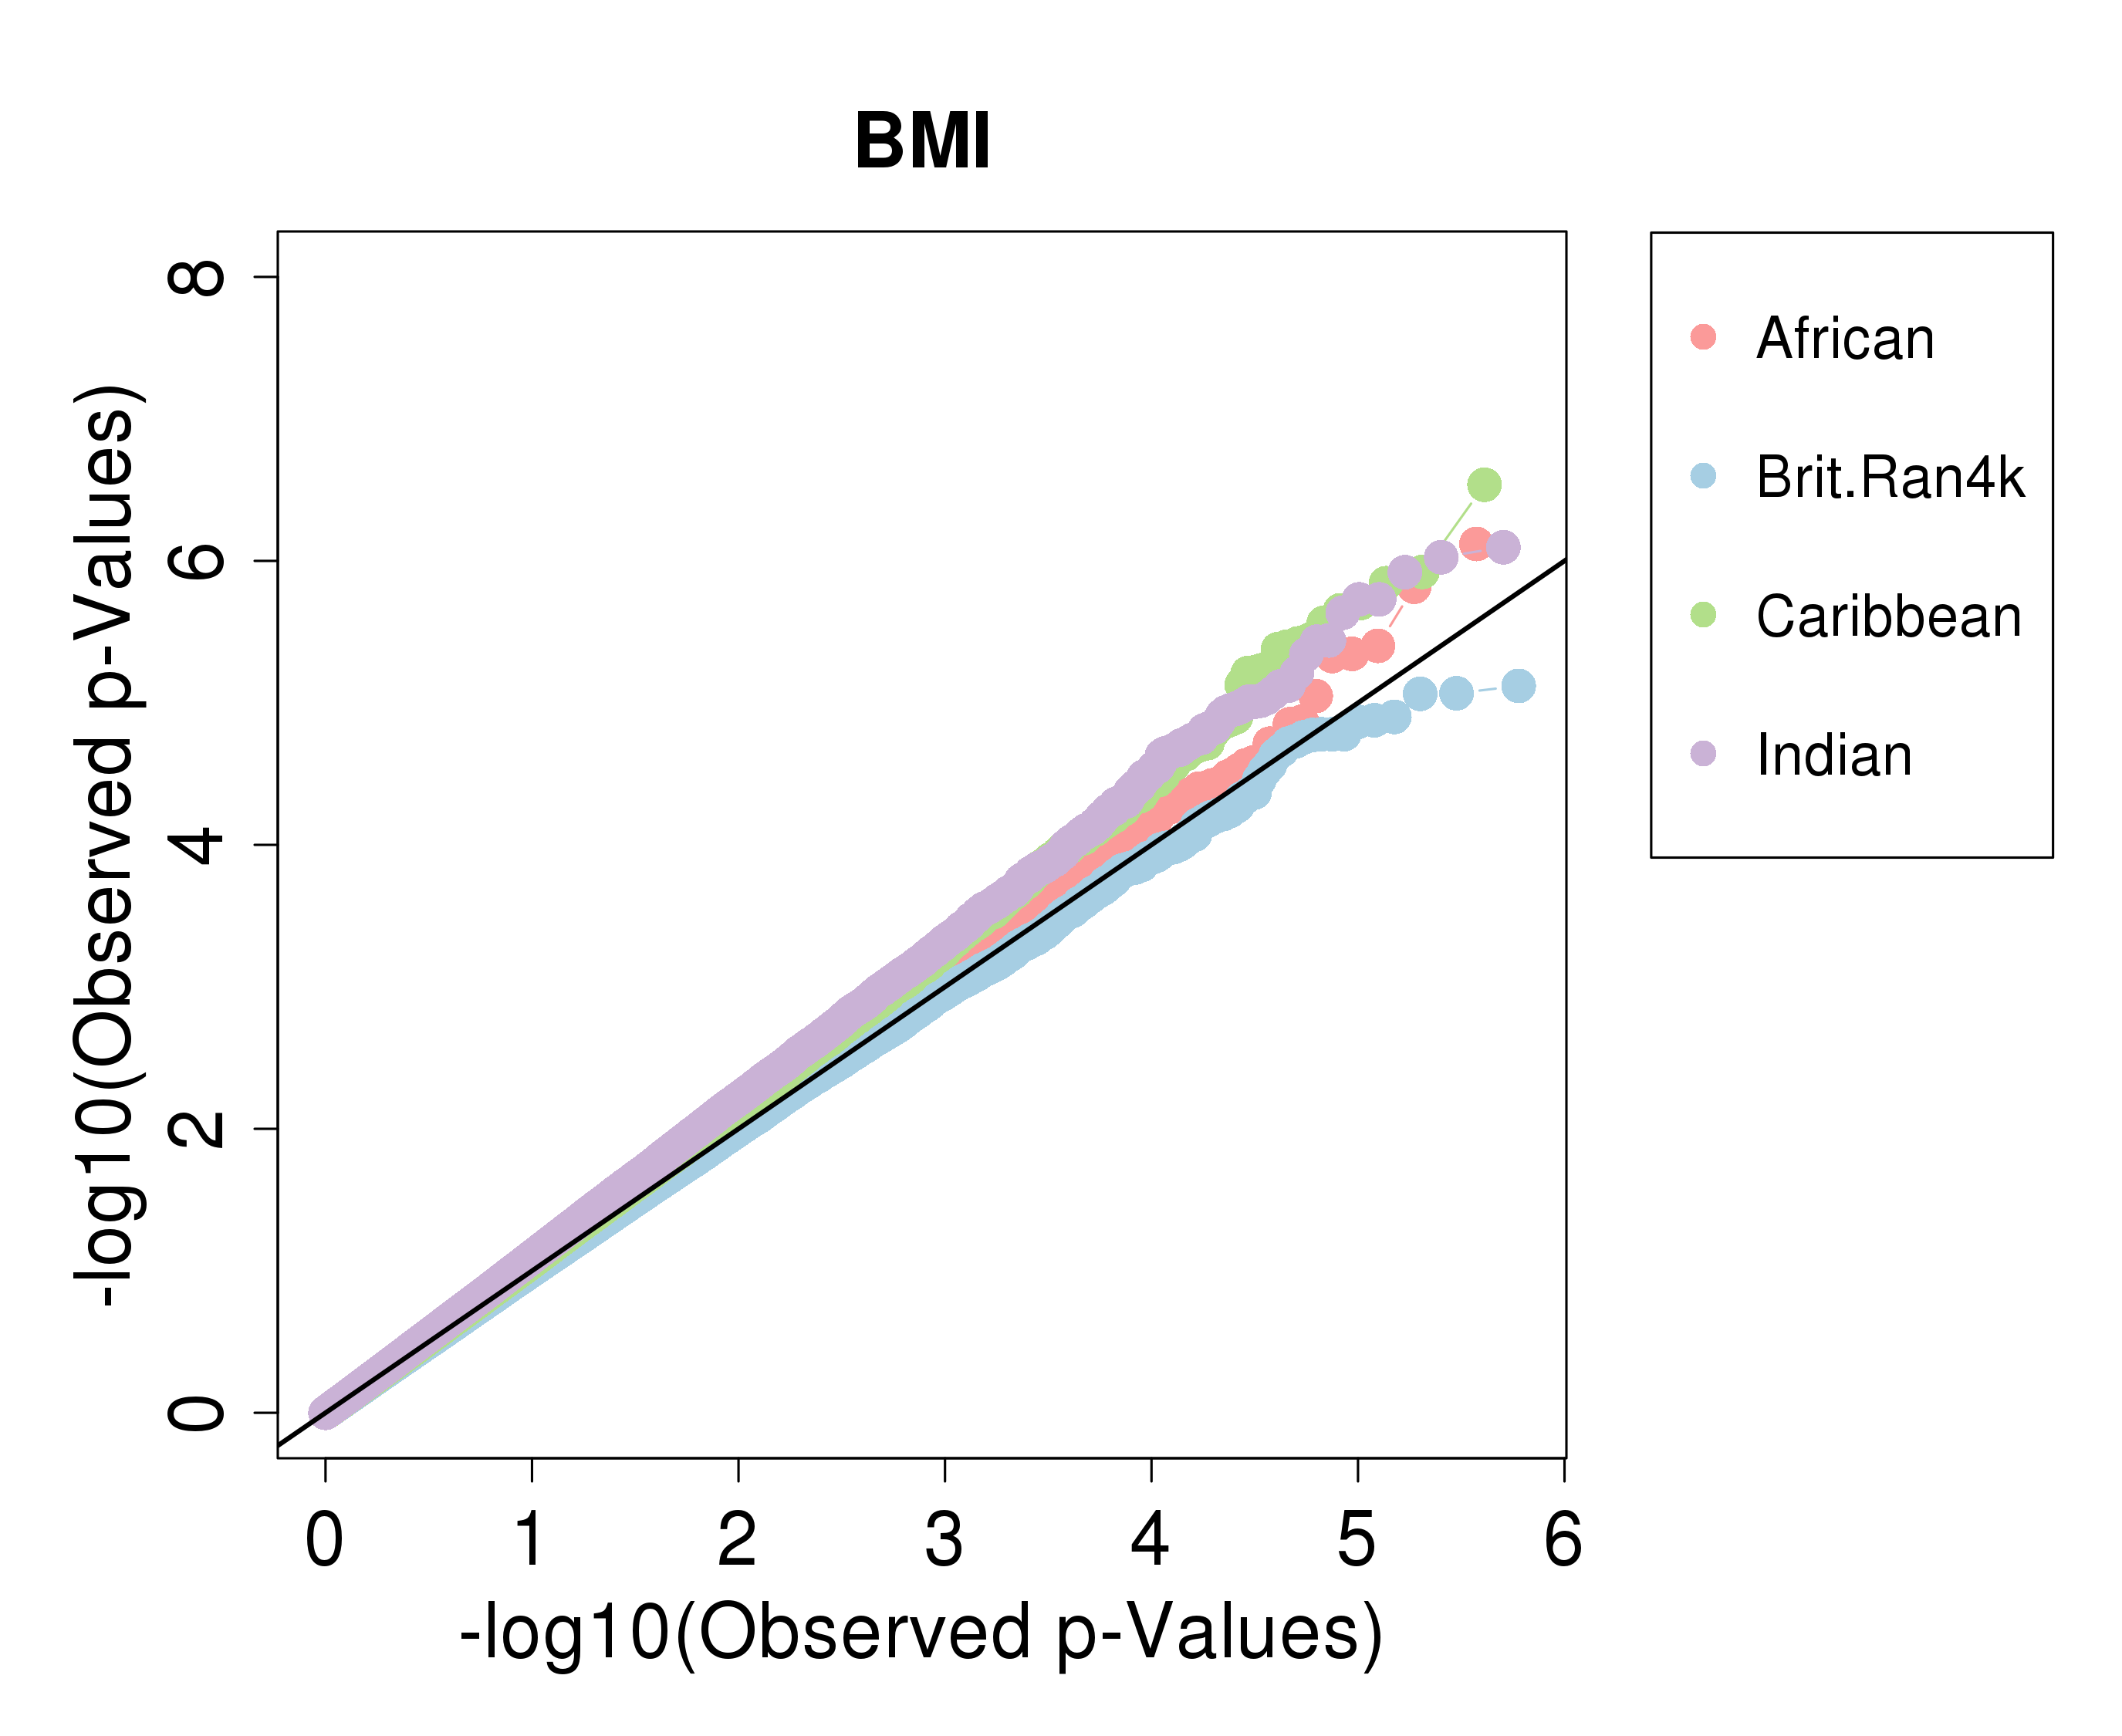
\includegraphics[scale=.35]{Images/Supp/InterPath_Supp_Figure_MAPIT_vs3_BMI.png}
\caption[TBD]{\textbf{MAPIT Results QQ-Plots}. Shown are QQ-plots of our results from running MAPIT on our four initial UKB population subsets in height and BMI. On the $x$-axis are the -$\log_{10}$ of our expected $p$-values and the on the $y$-axis are on the -$\log_{10}$ of our observed $p$-values. We observe weak signals of marginal epistasis across most of the population subsets in height and only a few potential weak signals in BMI. We do observe potential differences across population subsets. However, this lack of signal may be a product of our limited sample sizes, emphasizing the need to increase power through other means, such as by methodological improvements.}
\label{InterPath-Supp-Figure-MAPIT-BMI}
\end{figure}
\clearpage

\begin{figure}[htbp]
\centering
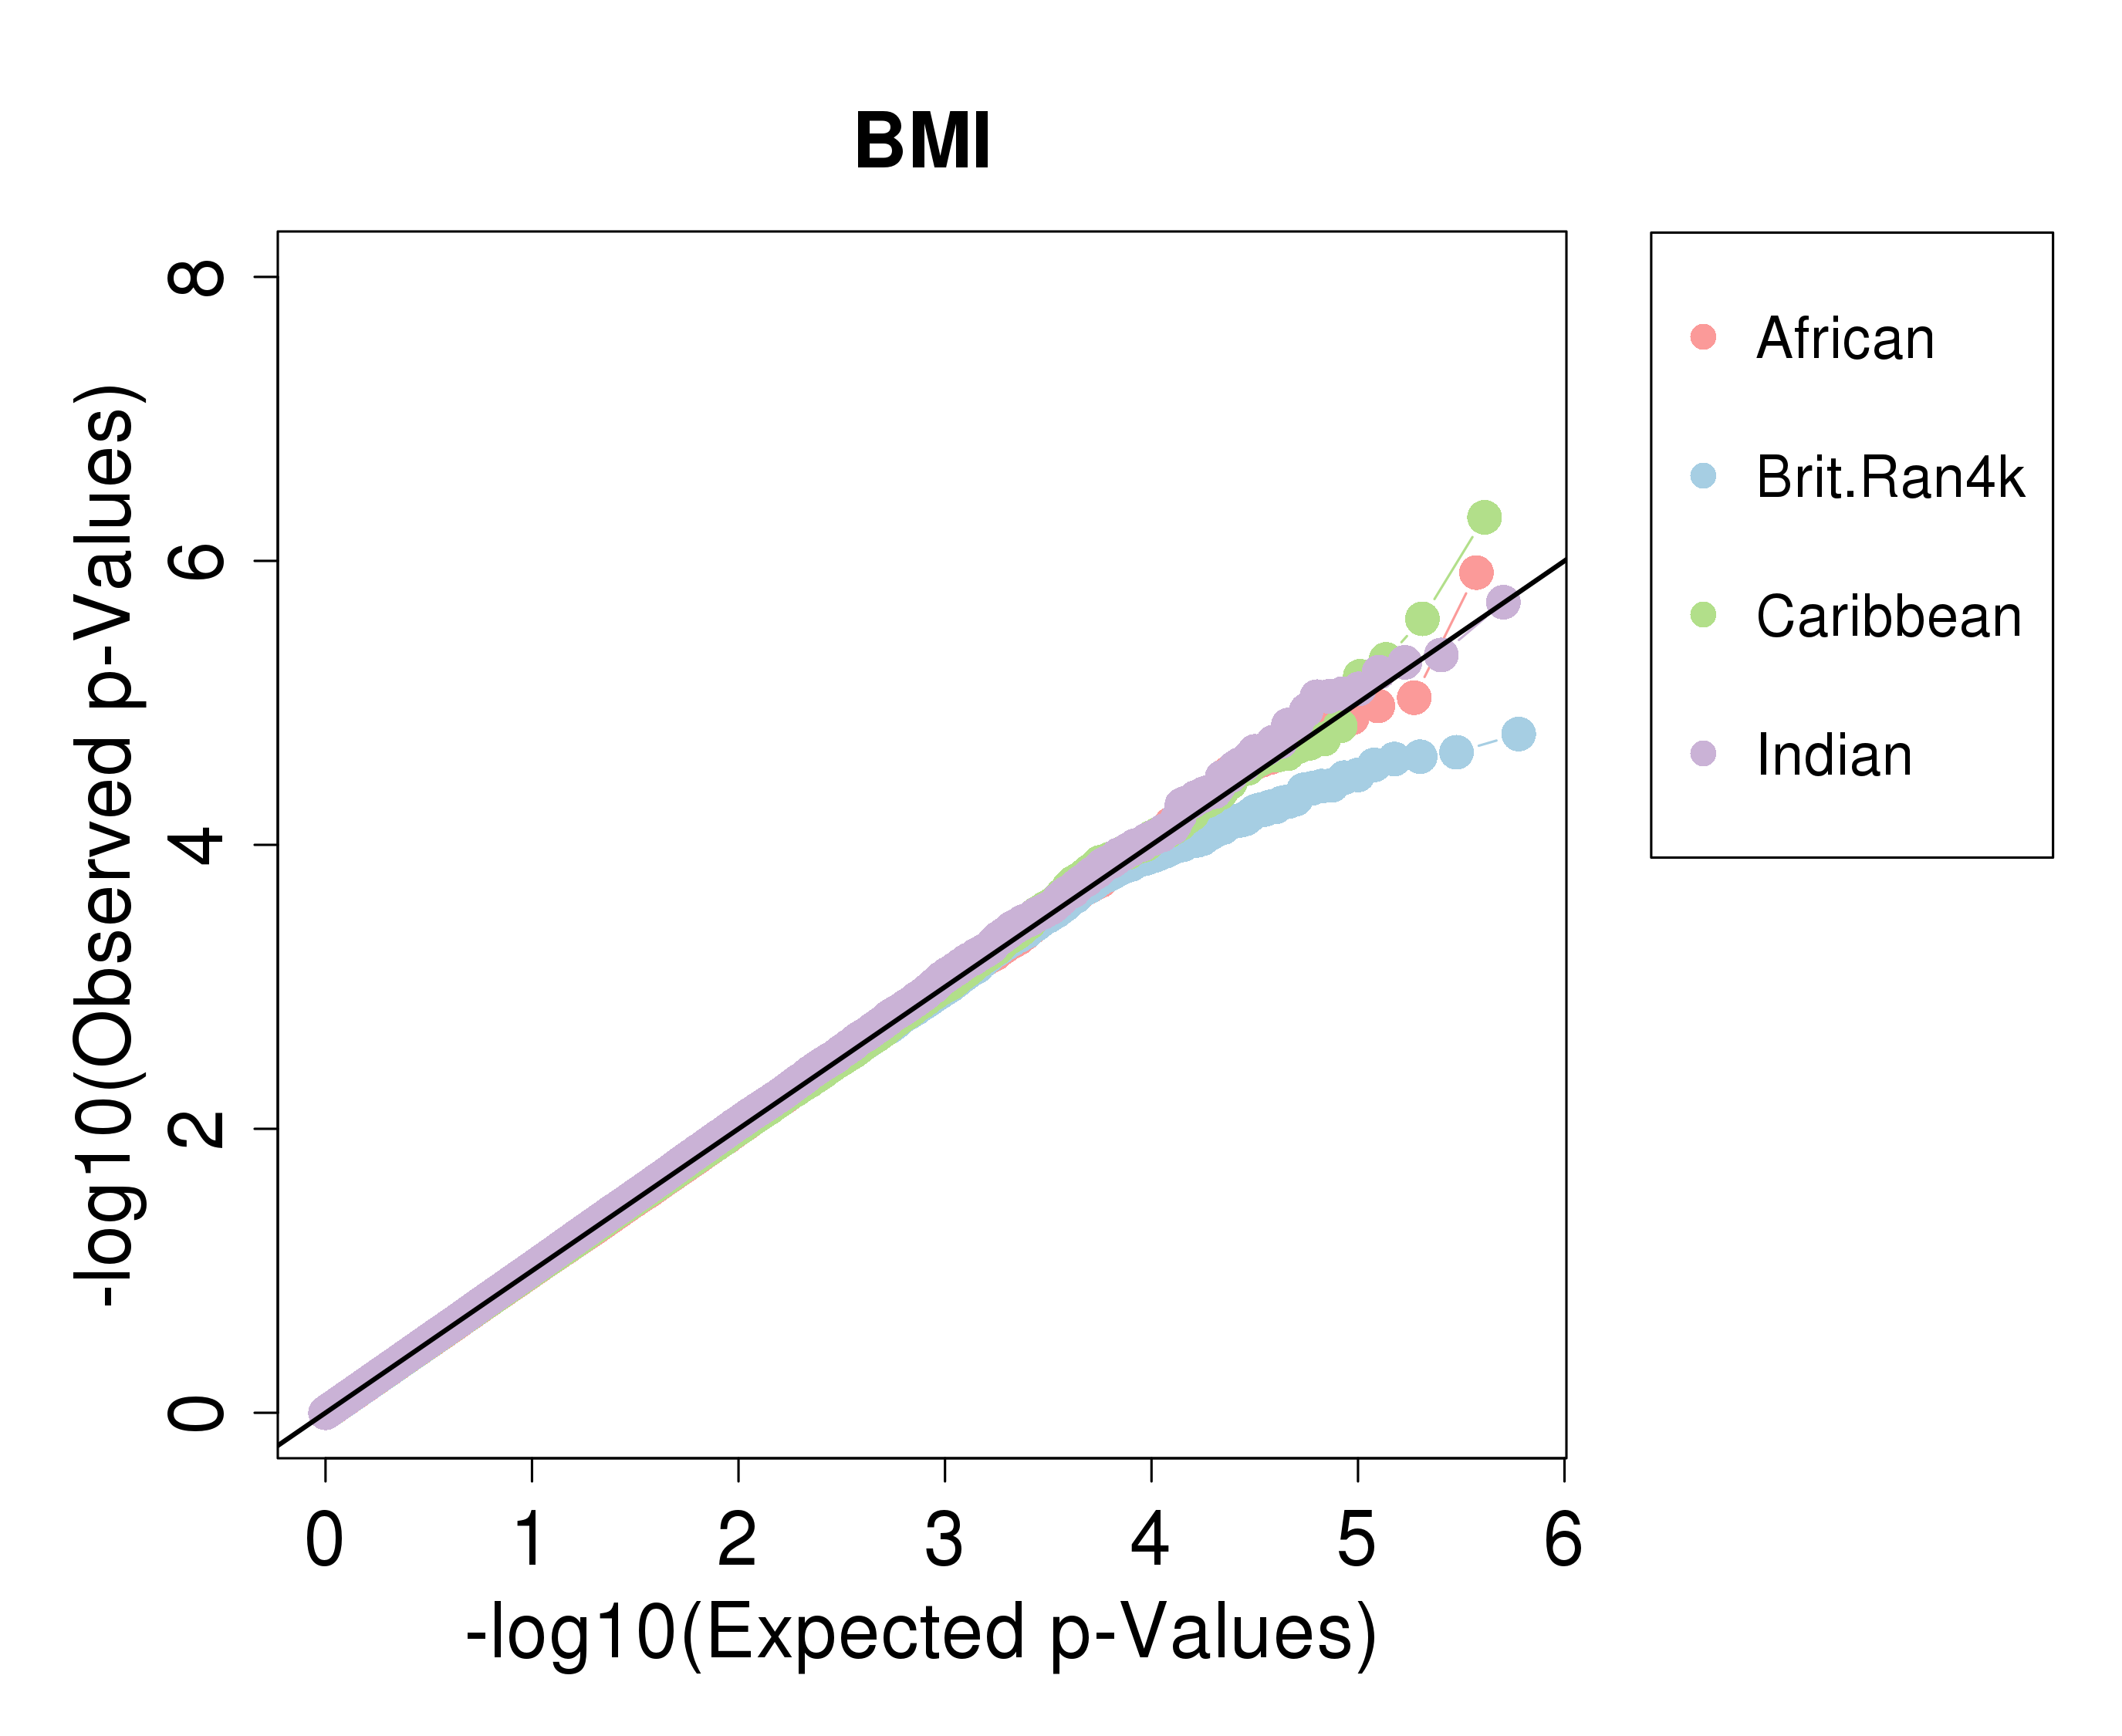
\includegraphics[scale=.35]{Images/Supp/InterPath_Supp_Figure_GWAS_vs2_BMI.png}
\caption[TBD]{\textbf{GWAS Results QQ-Plots}.}
\label{InterPath-Supp-Figure-GWAS-BMI}
\end{figure}
\clearpage

\begin{figure}[htbp]
\centering
\hspace*{-.75cm}
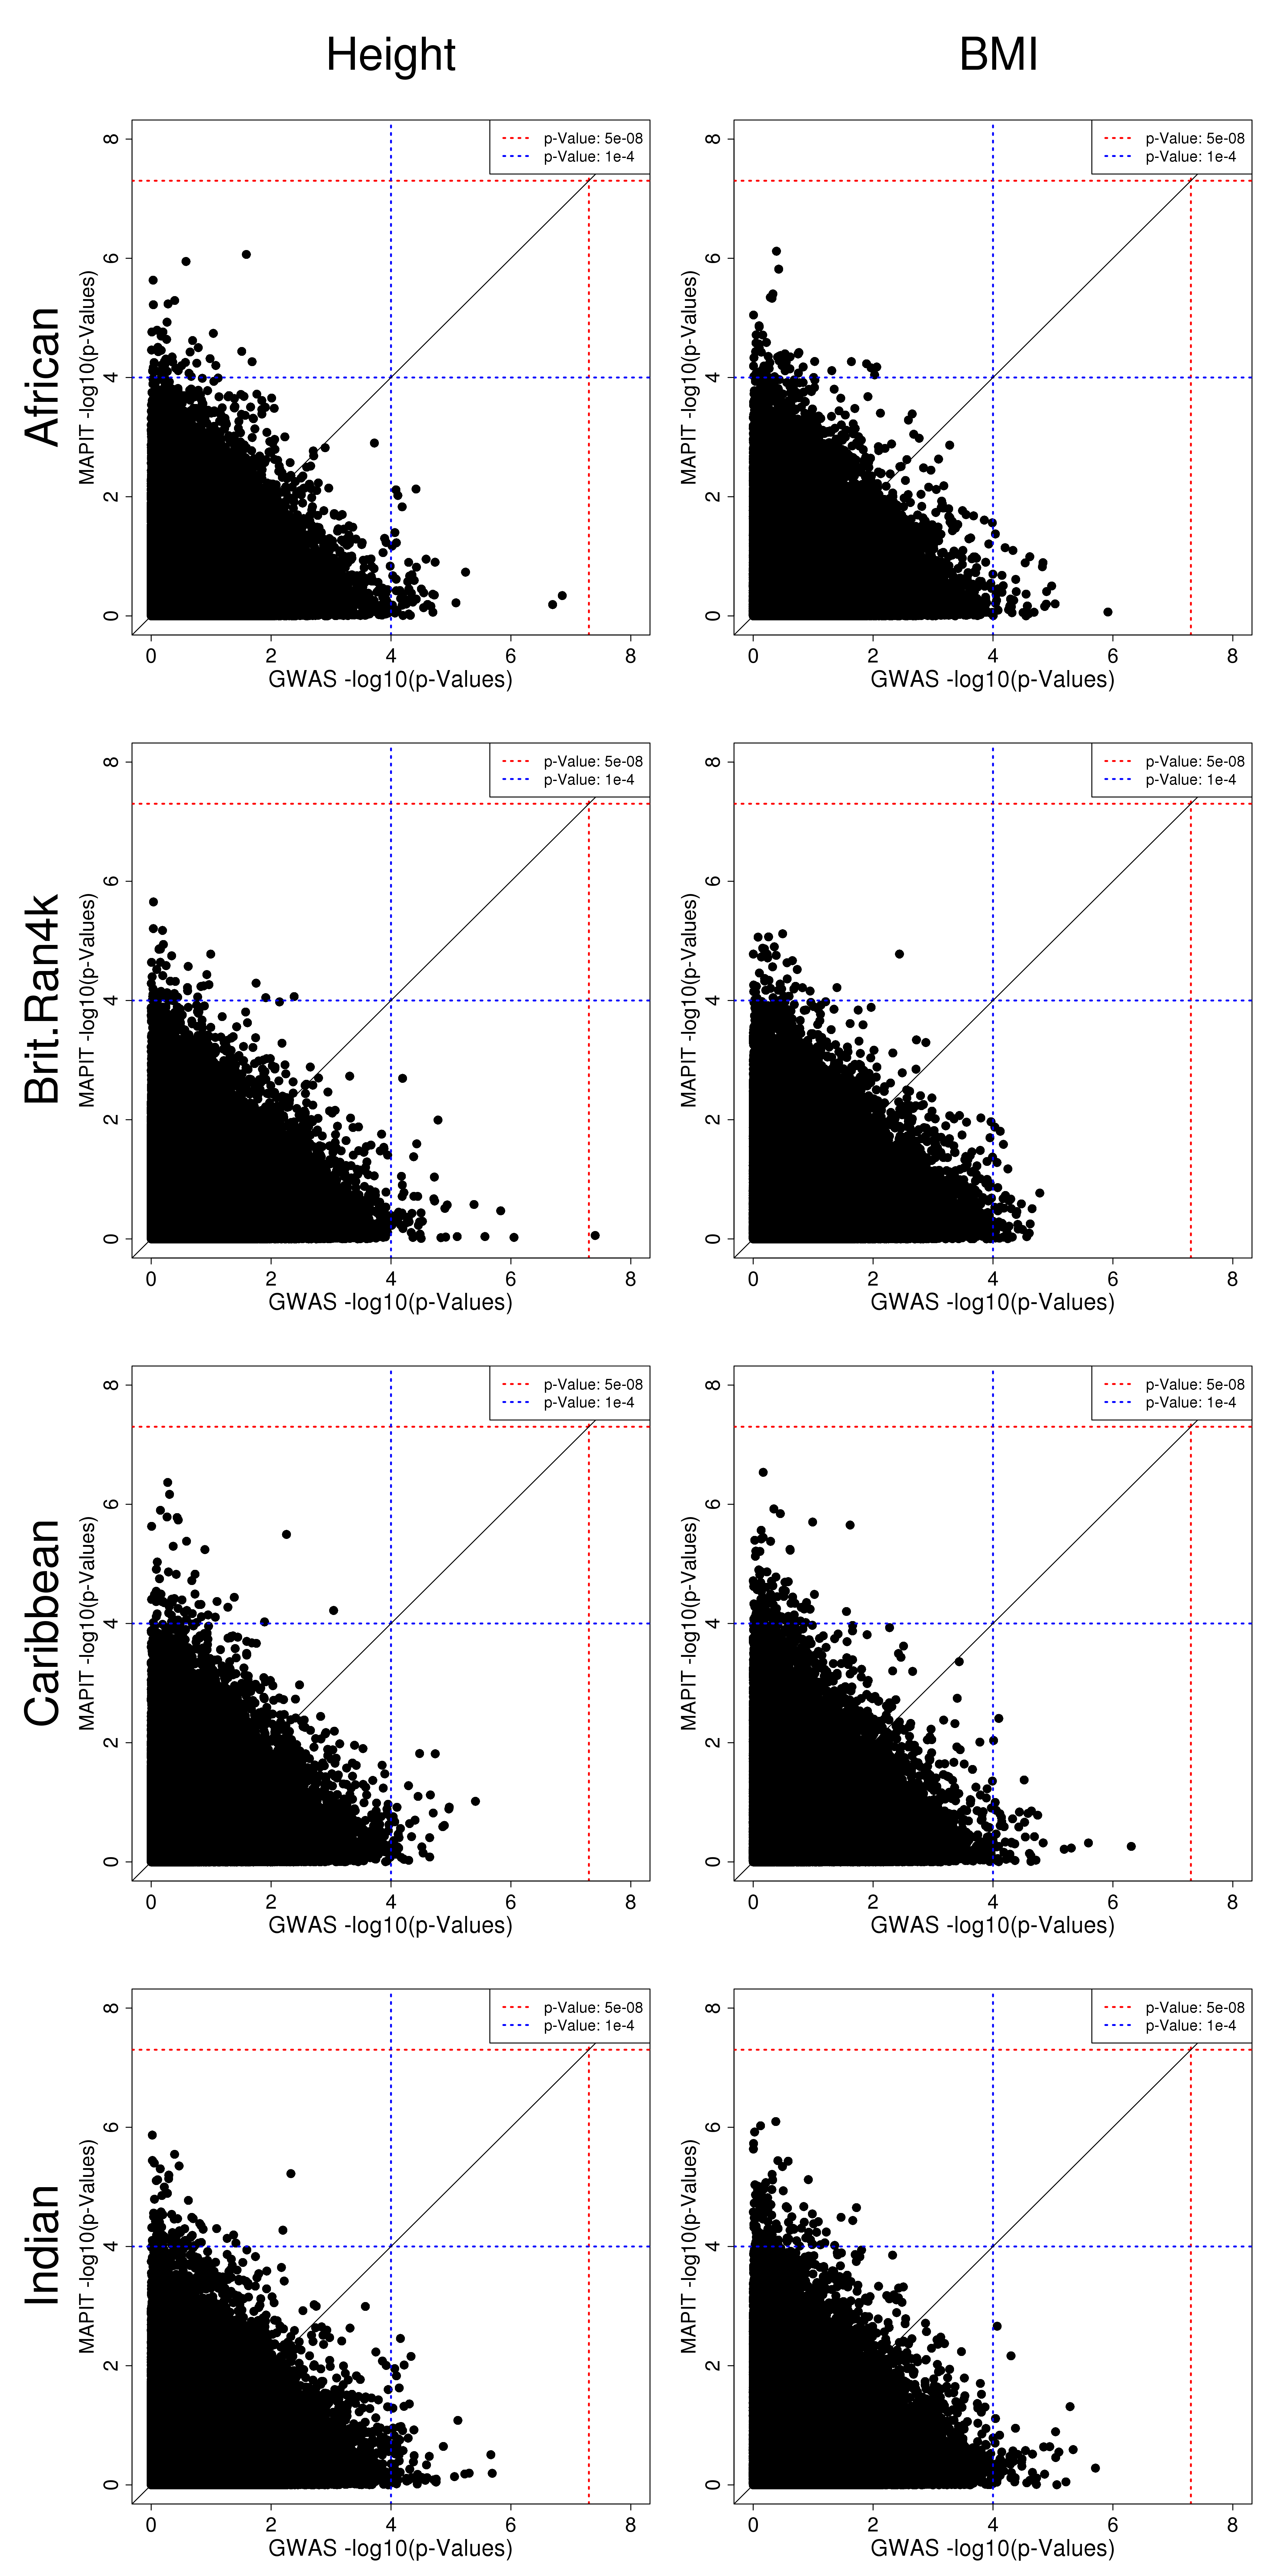
\includegraphics[scale=.3]{Images/Supp/InterPath_Supp_Figure_MAPITvsGWAS_vs2.png}
\caption[TBD]{\textbf{MAPIT vs. GWAS Results}.}
\label{InterPath-Supp-Figure-MAPITvsGWAS}
\end{figure}
\clearpage

\begin{figure}[htbp]
\centering
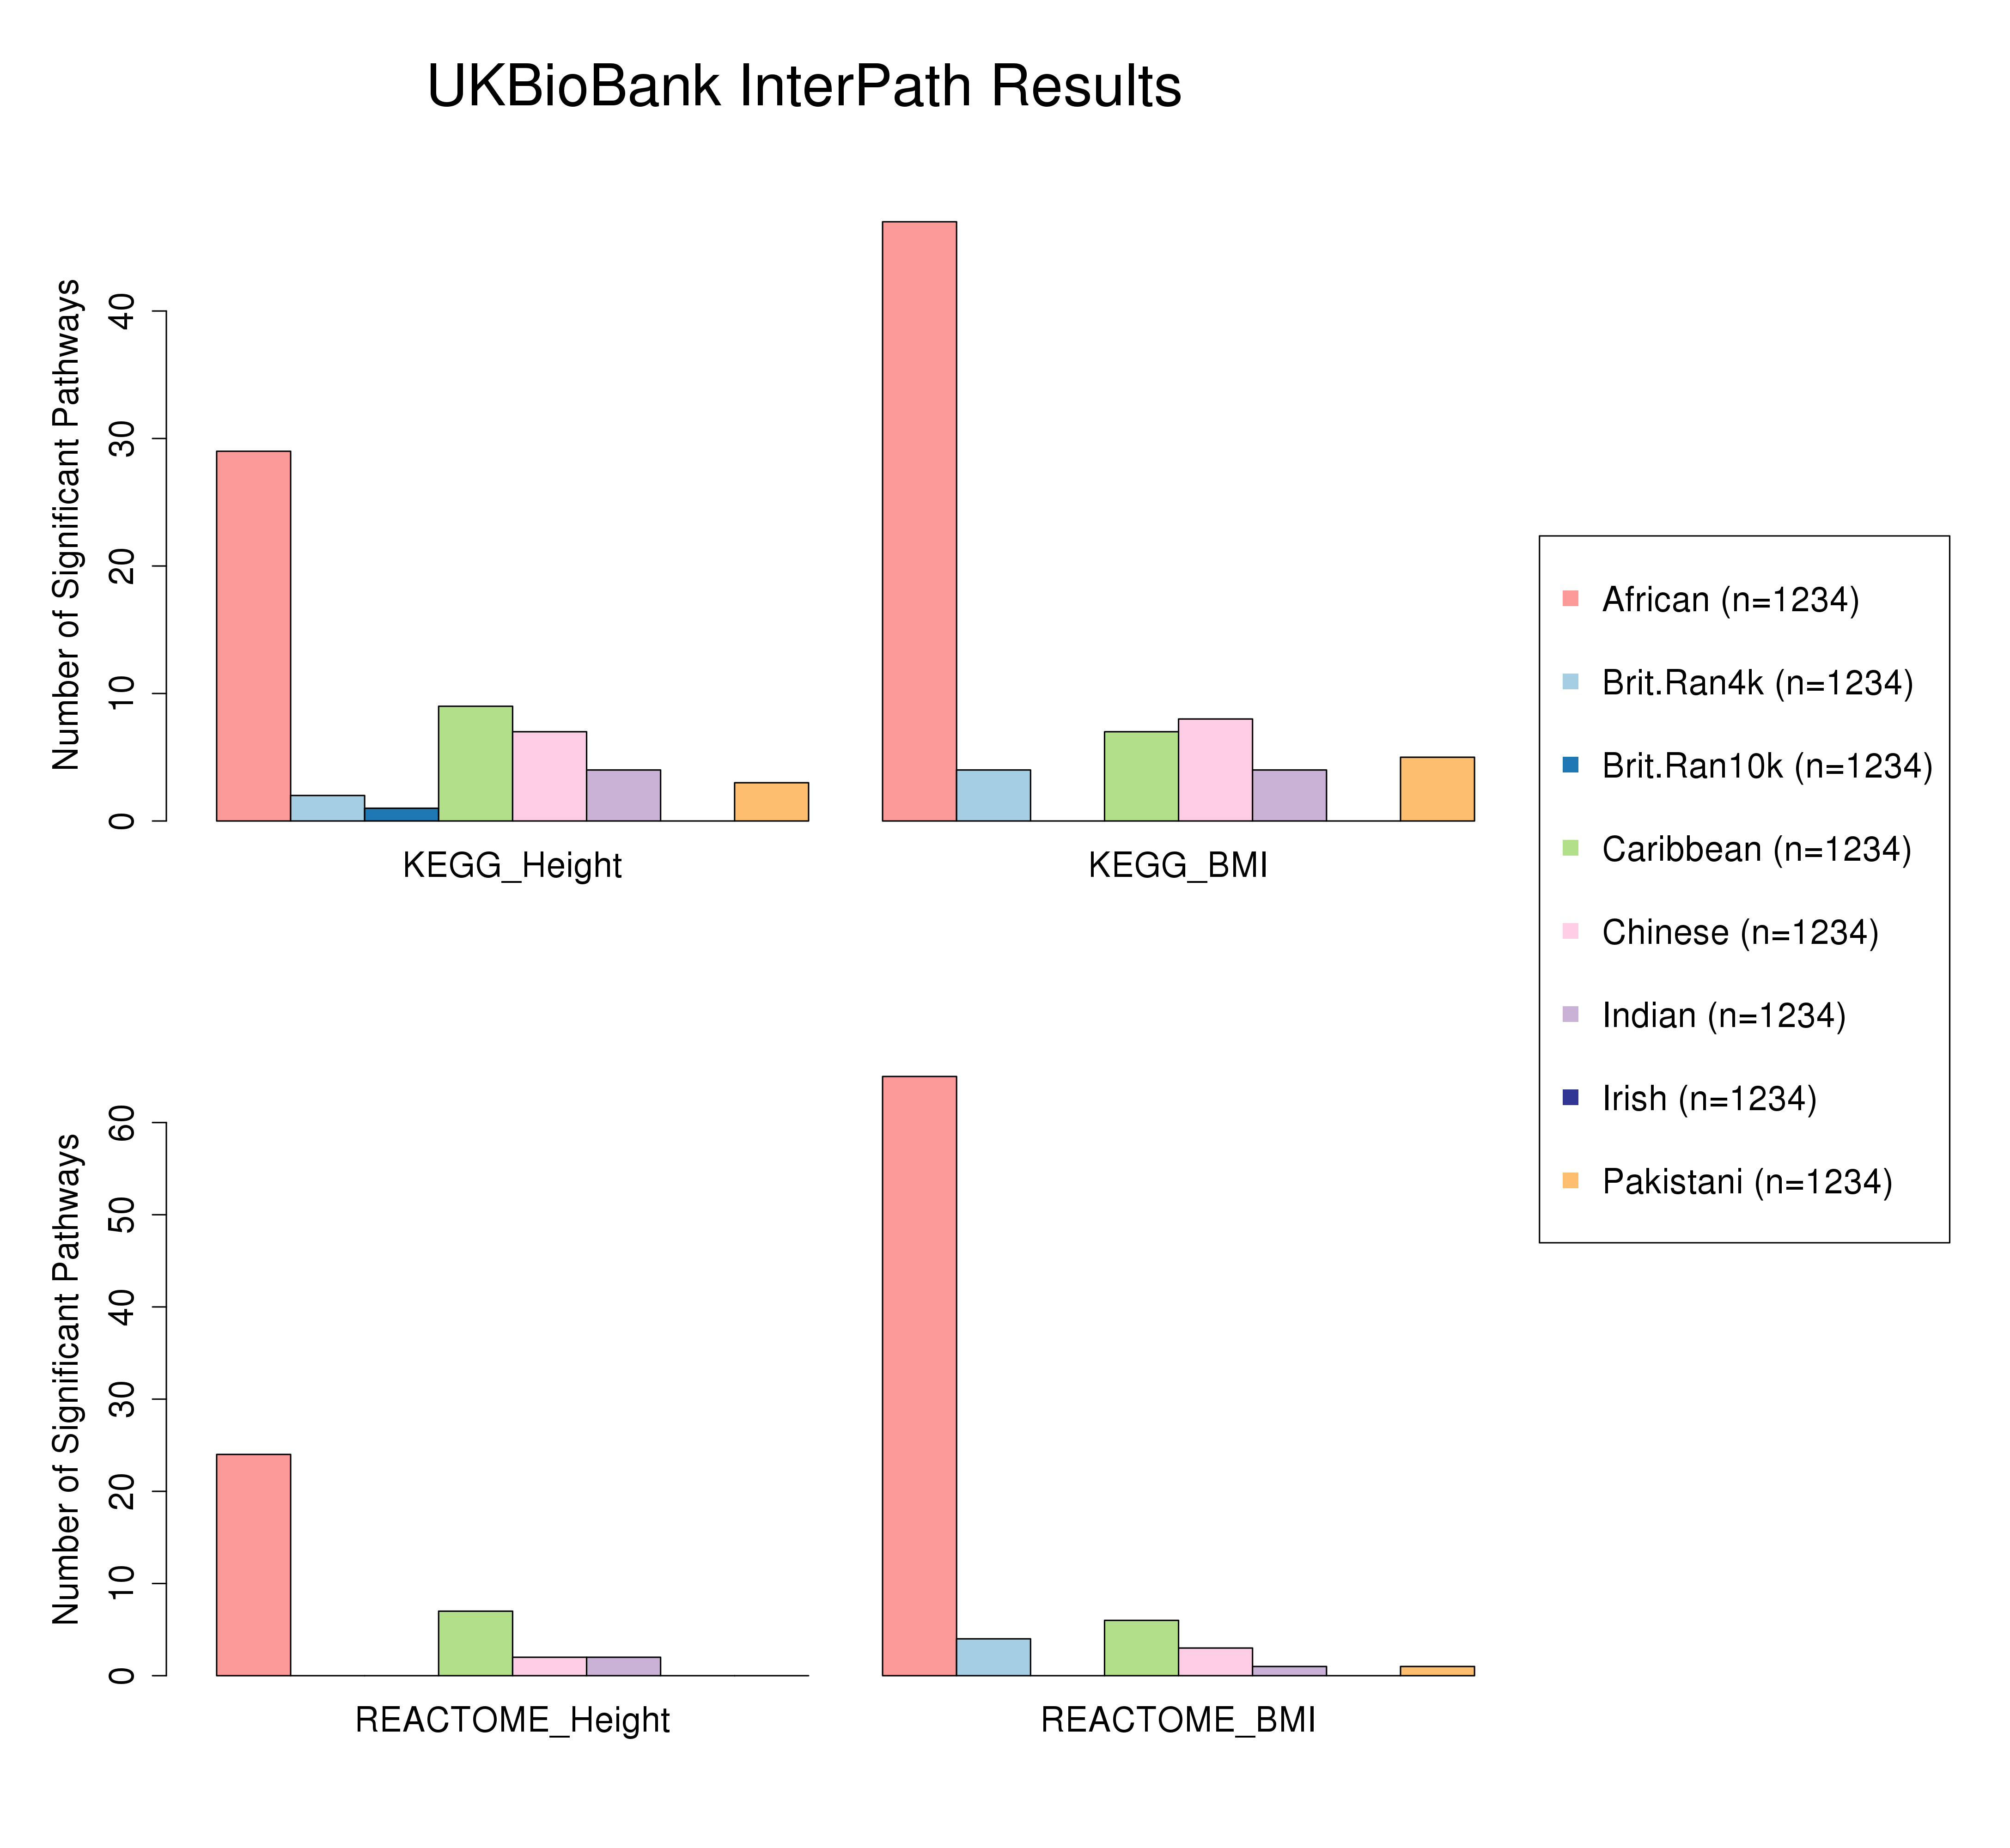
\includegraphics[scale=.35]{Images/Supp/InterPath_Supp_Figure_Barplots_vs1.png}
\caption[TBD]{\textbf{Number of Significant Pathways from Running MAPIT-R on UKB subsets}. Shown are the number of significant pathways found from running MAPIT-R on each of our expanded collection of UKB population subsets using height and BMI in the KEGG database (REACTOME results can be found in Supplementary Figure XX). A pathway is considered significant if its MAPIT-R $p$-value is below XXX (.05 / XXX, the number of KEGG pathways tested). We find that the African population far and away has the largest number of significant pathways, both for each phenotype and for each pathway database. But in general we also tend to see significant pathways moreso in non-European populations than European populations.}
\label{InterPath-Supp-Figure-Barplots-All}
\end{figure}
\clearpage

\begin{figure}[htbp]
\centering
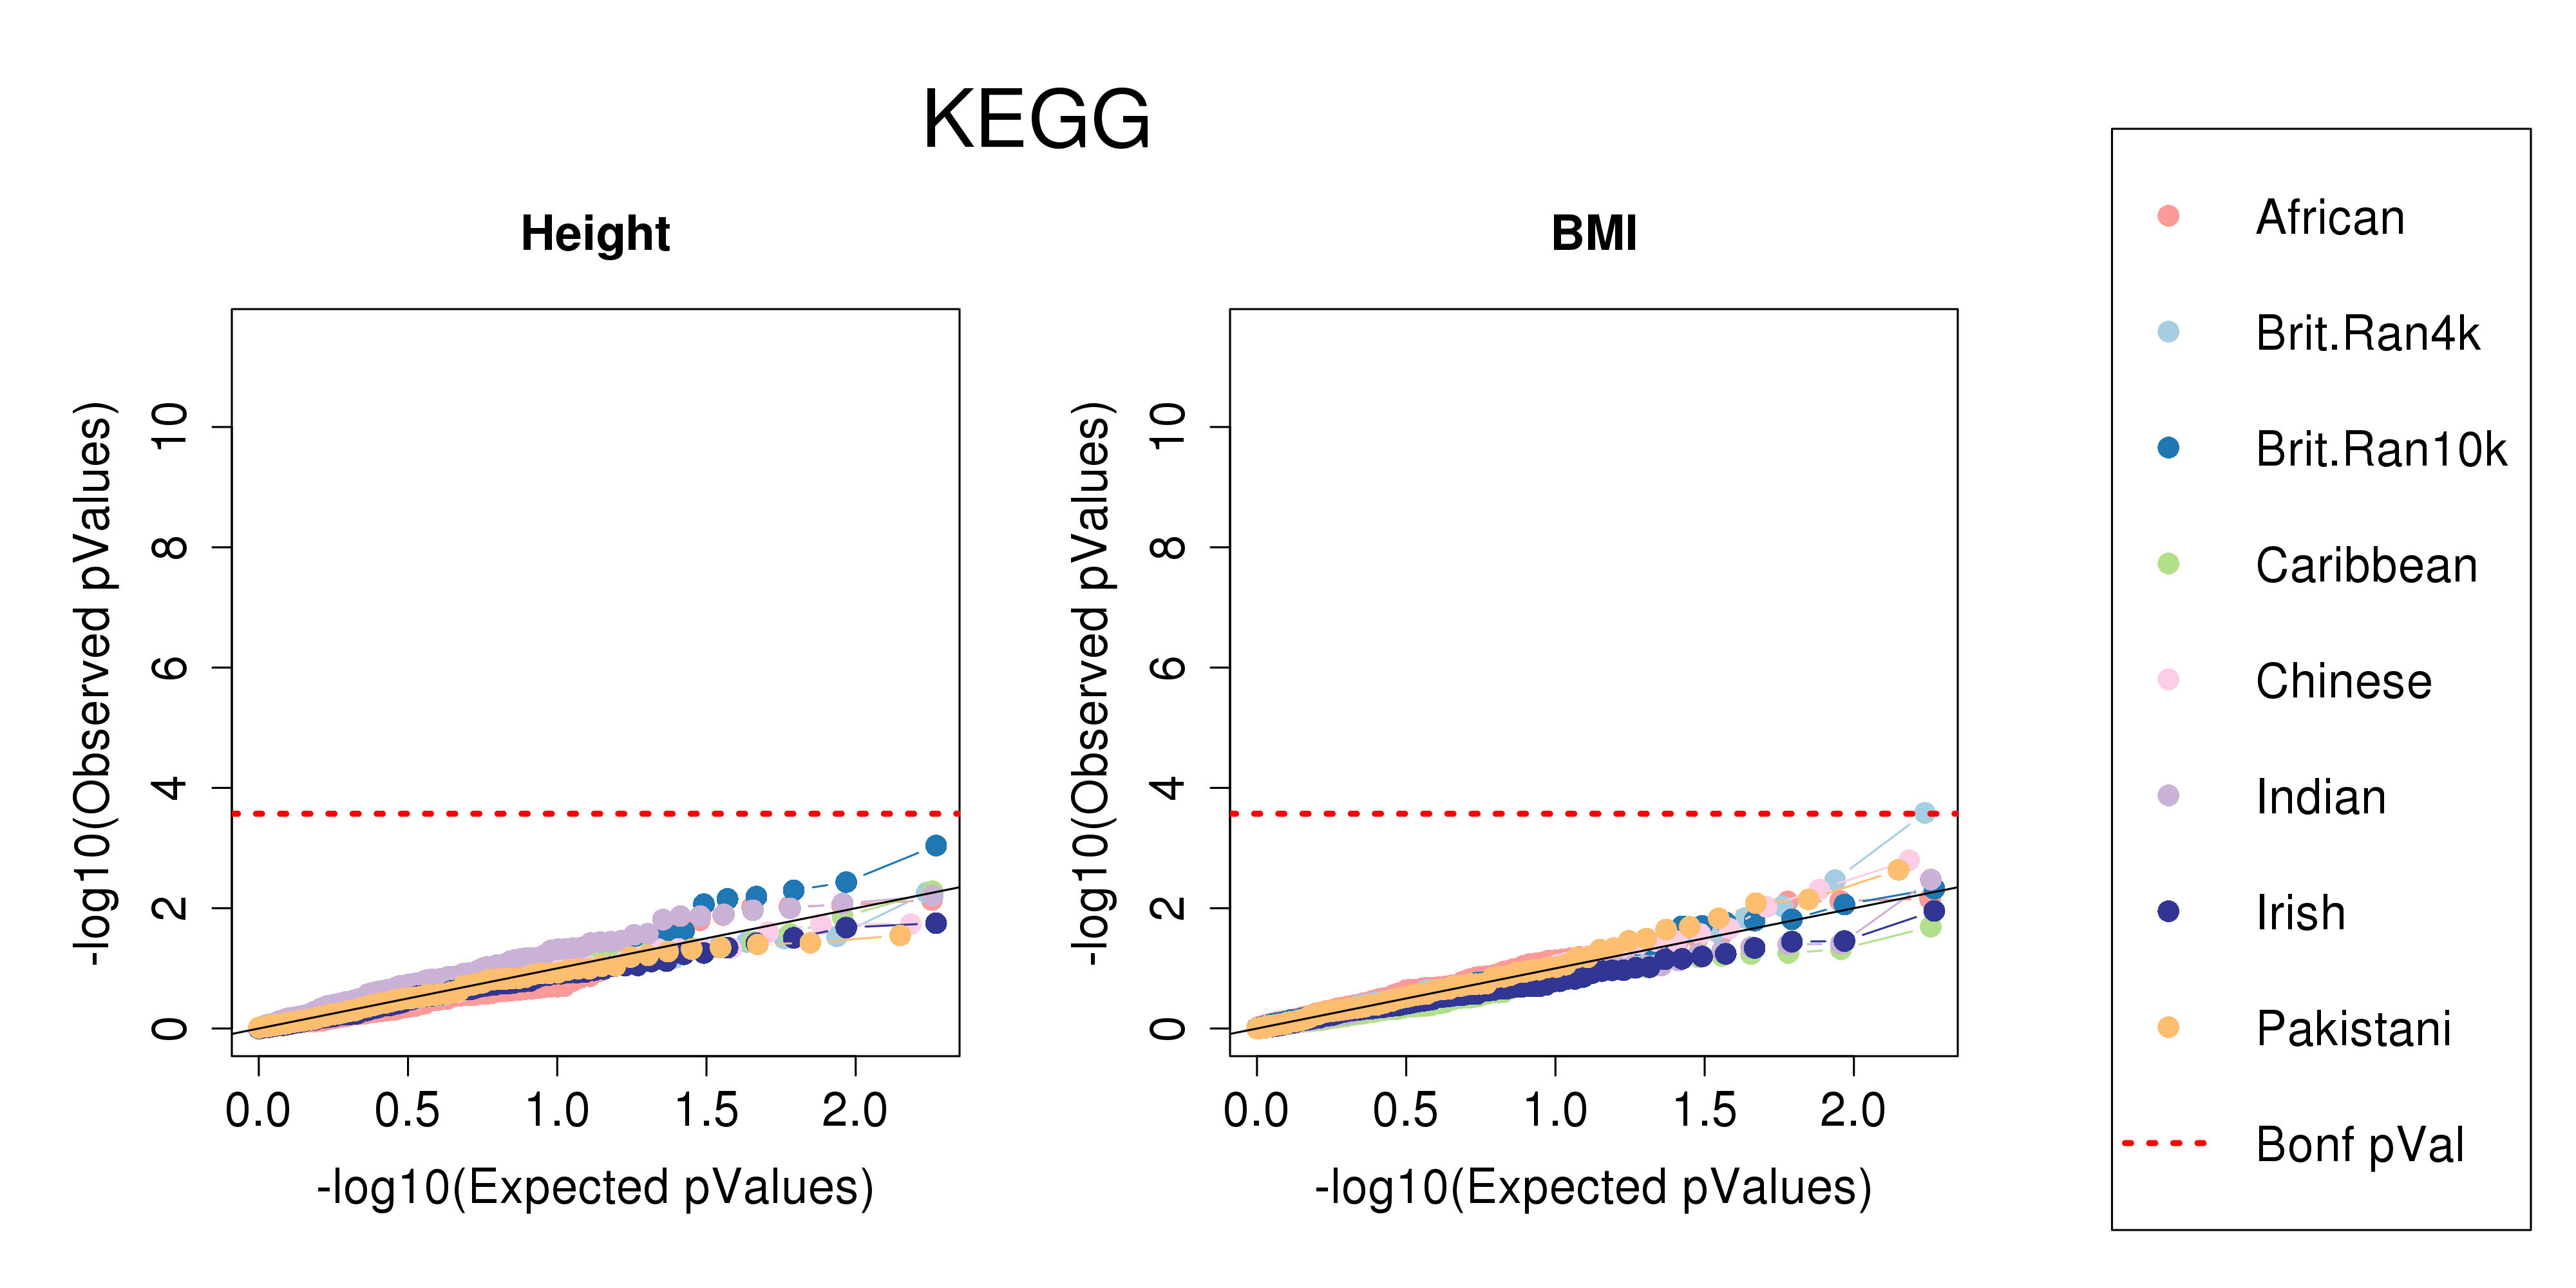
\includegraphics[scale=.35]{Images/Supp/InterPath_Supp_Figure_perm1_QQPlots_KEGG_vs1.png}
\caption[TBD]{\textbf{MAPIT-R Phenotype Permutation QQ-Plots}. Shown are QQ-plots for running MAPIT-R using a single, permuted version of the phenotypes for both Height and BMI with the KEGG pathways. Phenotypes were permuted within each population subset. Shown on the $x$-axis are the -$\log_{10}$ of our expected $p$-values and the on the $y$-axis are on the -$\log_{10}$ of our observed $p$-values. The dotted red line is our Bonferroni-corrected $p$-value threshold (.05 / XX KEGG pathways). We find across all population subsets that MAPIT-R displays the null behavior as expected when using permuted phenotypes.}
\label{InterPath-Supp-Figure-perm1-QQPlots-KEGG}
\end{figure}
\clearpage

\begin{figure}[htbp]
\centering
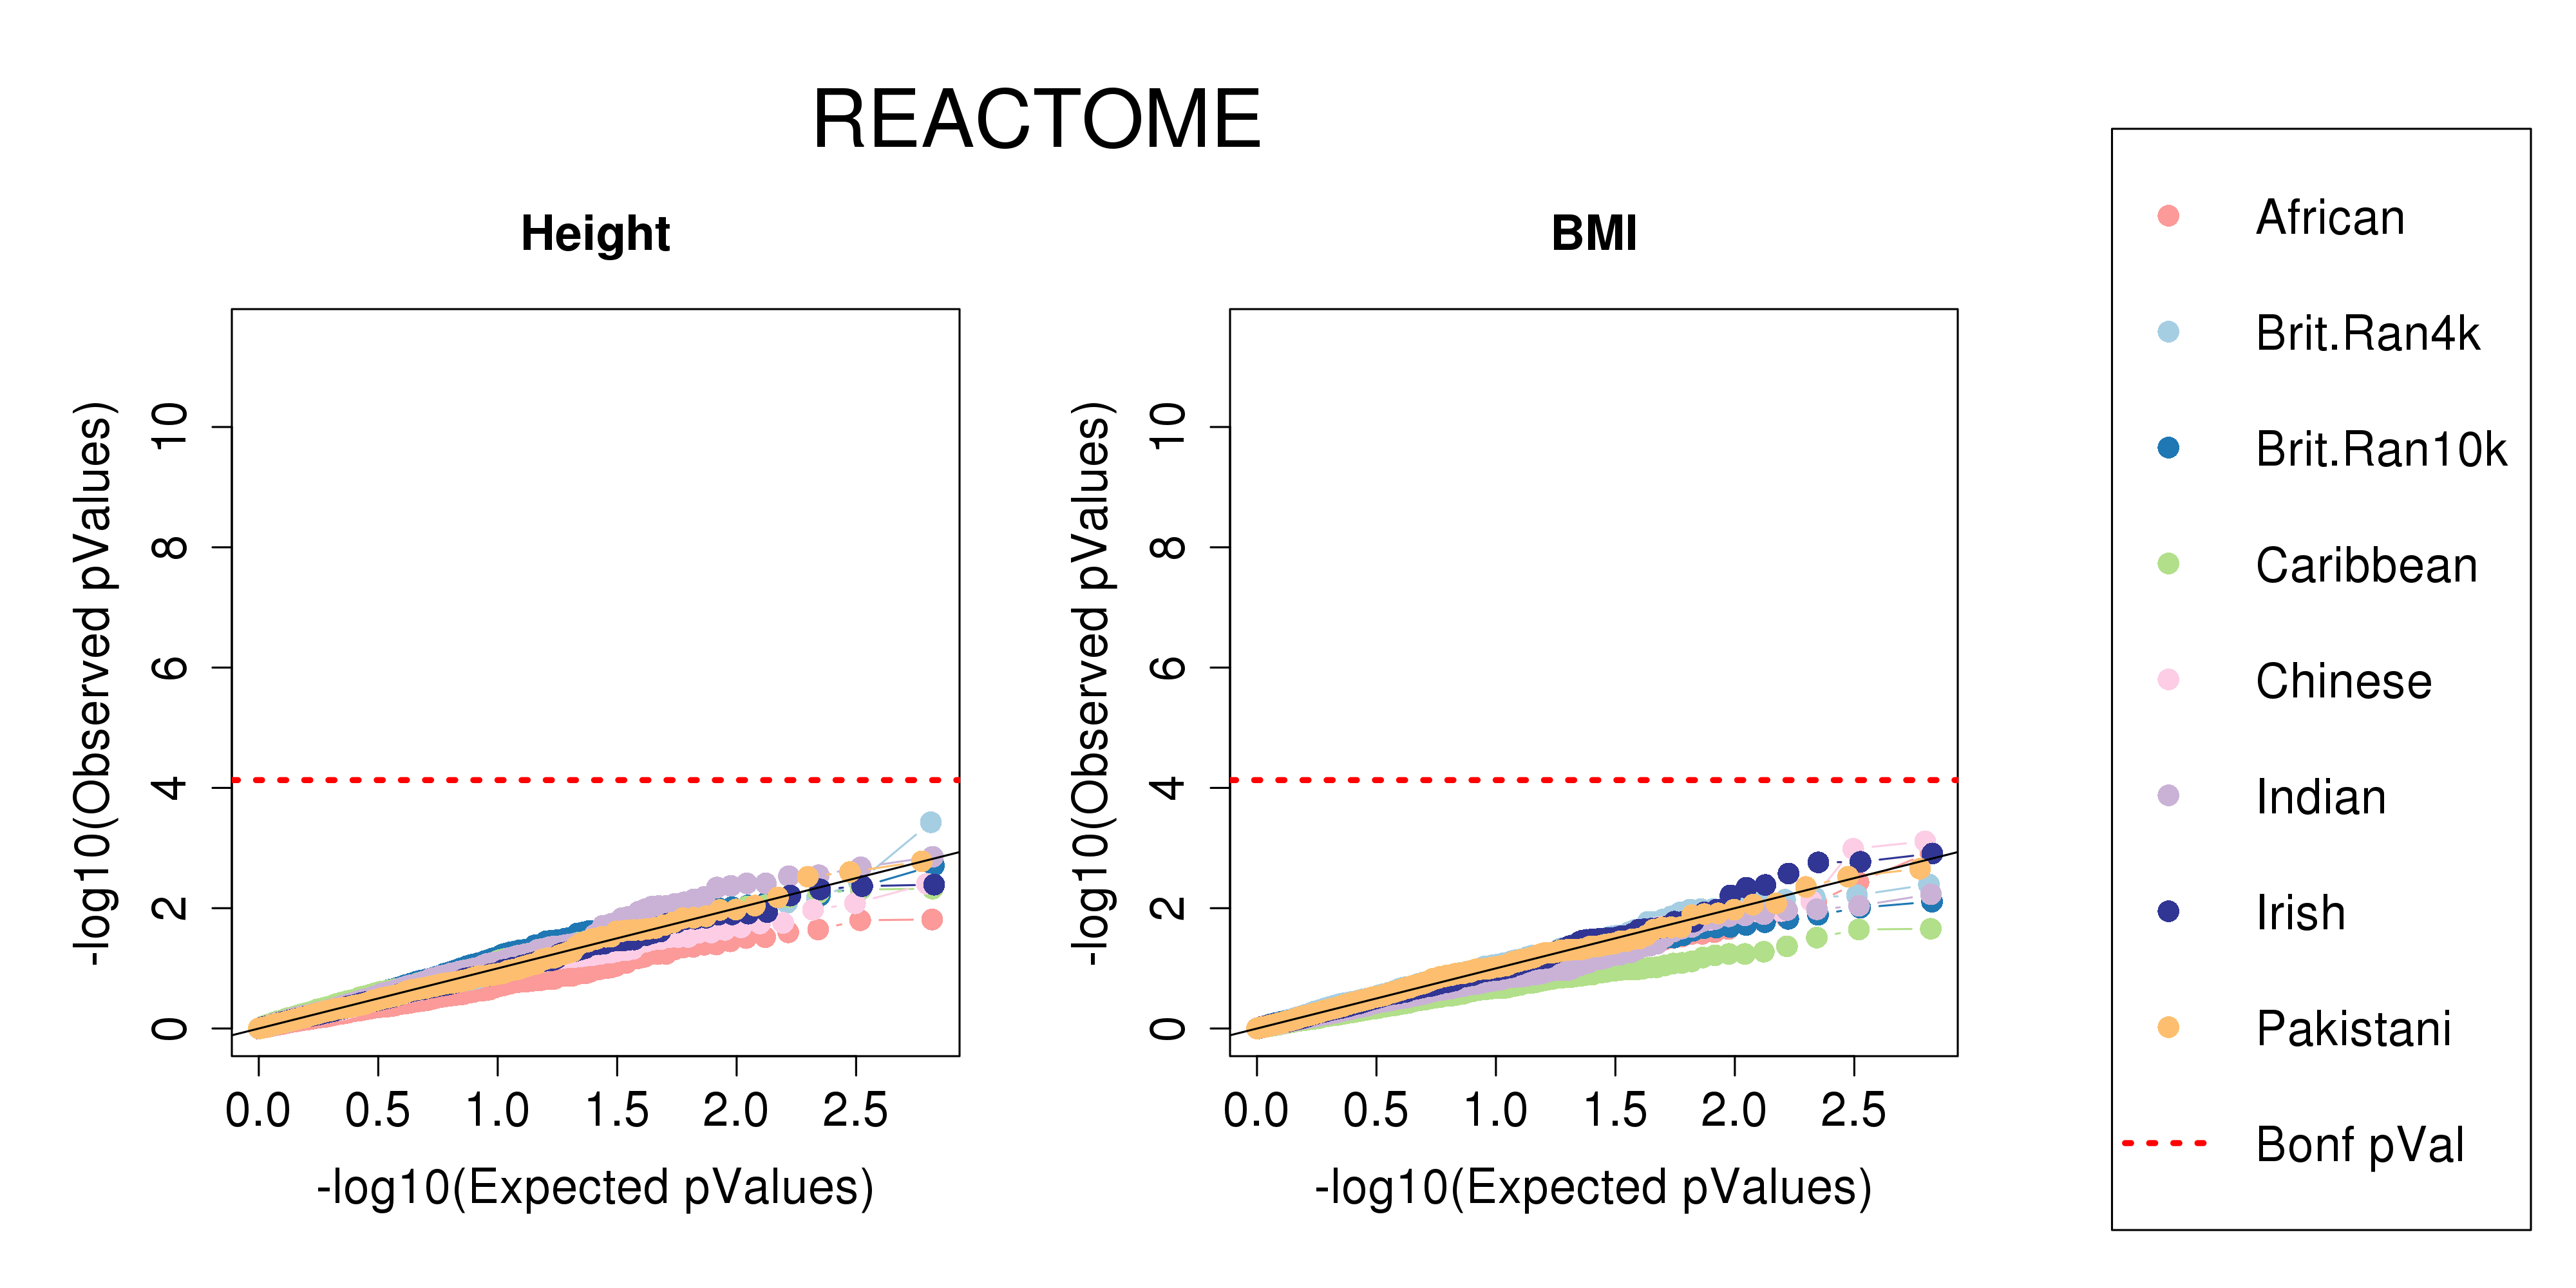
\includegraphics[scale=.35]{Images/Supp/InterPath_Supp_Figure_perm1_QQPlots_REACTOME_vs1.png}
\caption[TBD]{\textbf{TBD}. \\ Same as above (will be put in Supplementary).}
\label{InterPath-Supp-Figure-perm1-QQPlots-REACTOME}
\end{figure}
\clearpage

\begin{figure}[htbp]
\centering
\includegraphics[scale=.15]{Images/Supp/InterPath_Supp_Figure_pValHists_vs2.png}
\caption[TBD]{\textbf{TBD}. \\ Placeholder.}
\label{InterPath-Supp-Figure-10perms-pValHists}
\end{figure}
\clearpage

\begin{figure}[htbp]
\centering
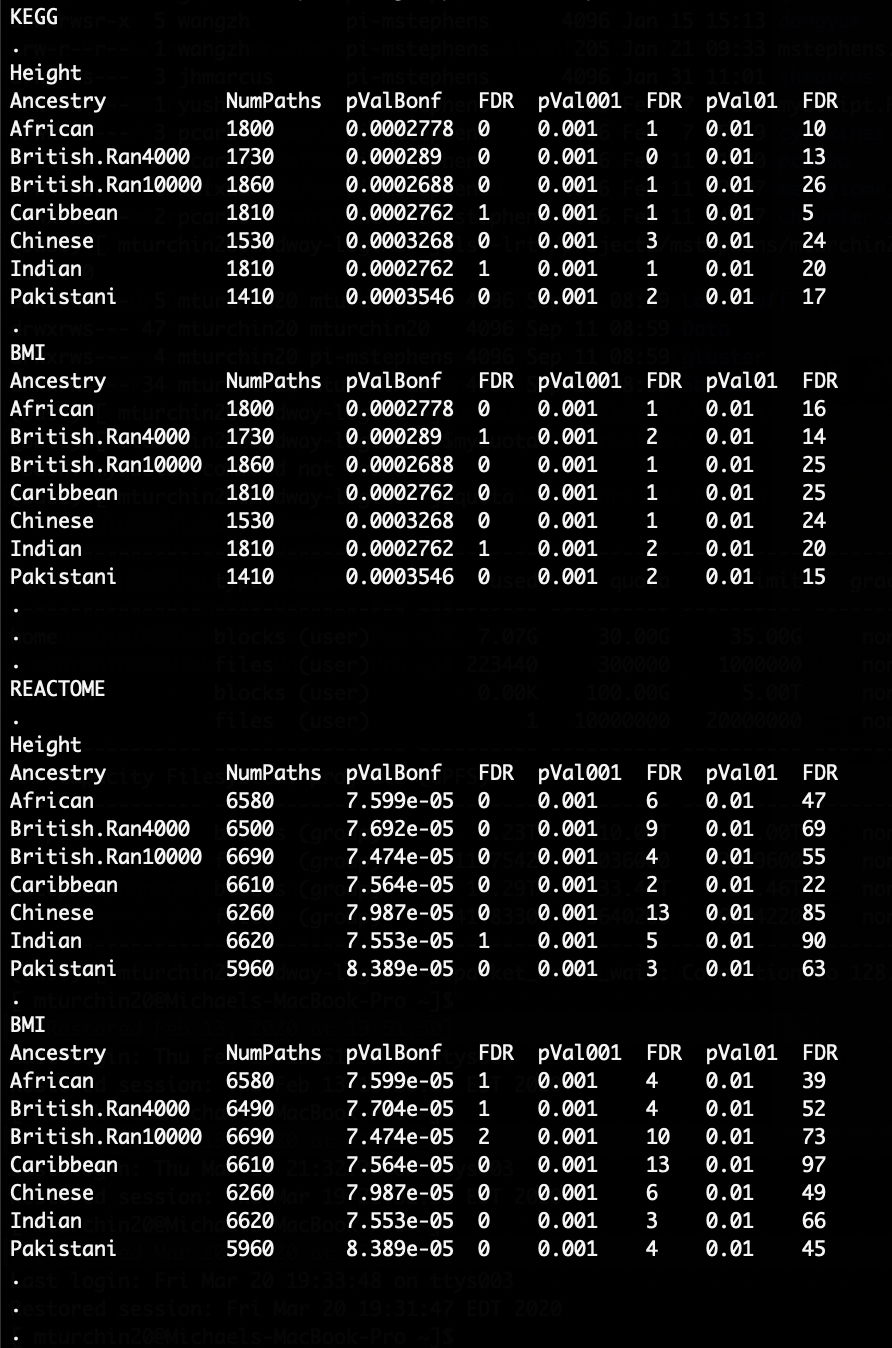
\includegraphics[scale=1.5]{Images/Supp/InterPath_Supp_Figure_FDRs_AllPops_vs1.png}
\caption[TBD]{\textbf{TBD}. }
\label{InterPath-Supp-Figure-FDR-AllPops}
\end{figure}
\clearpage

\begin{figure}[htbp]
\centering
\includegraphics[scale=.15]{Images/Supp/InterPath_Supp_Figure_pValsVsNumSNPs_vs1.png}
\caption[TBD]{\textbf{MAPIT-R $p$-values Versus Number of SNPs in a Pathway}. \\ Shown is the relationship between MAPIT-R $p$-values and the number of SNPs found in a tested pathway across all populations in height and BMI within KEGG. Shown on the $x$-axis is the number of SNPs that were included for a given pathway and on the $y$-axis is shown that pathway's MAPIT-R -$\log_{10}$ $p$-value. As expected, we find a generally positive relationship between these two variables -- in other words, the more SNPs that are included the more likely it is that MAPIT-R will have a more significant $p$-value. We also find, however, that it is not simply the SNPs counts that are driving this signal; looking at this same comparison within the permuted phenotype analyses we find barely any positive relationship between SNP counts per pathway and a pathway's MAPIT-R -$\log_{10}$ $p$-value (Supplementary Figure \ref{InterPath-Supp-Figure-pValsVsNumSNPs-perm1}}
\label{InterPath-Supp-Figure-pValsVsNumSNPs}
\end{figure}
\clearpage

%\begin{figure}[htbp]
%\centering
%\includegraphics[scale=.15]{Images/Supp/InterPath_Supp_Figure_pValsVsNumSNPs_perm1_vs1.png}
%\caption[TBD]{\textbf{MAPIT-R $p$-values Versus Number of SNPs in a Pathway, Permuted Phenotypes}. \\ Shown is the relationship between MAPIT-R $p$-values and the number of SNPs found in a tested pathway across all populations in permuted height and BMI within KEGG. Shown on the $x$-axis is the number of SNPs that were included for a given pathway and on the $y$-axis is shown that pathway's MAPIT-R -$\log_{10}$ $p$-value. Unlike with the observed data (Figure \ref{InterPath-Supp-Figure-pValsVsNumSNPs}), we do not see a relationship between the number of SNPs included in a pathway and that pathway's -$\log_{10}$ MAPIT-R $p$-value. This shows that while having more SNPs allows MAPIT-R to generate more power to detect epistatic interactions, our significant results are not due solely to having more SNPs.}
%\label{InterPath-Supp-Figure-pValsVsNumSNPs-perm1}
%\end{figure}
%\clearpage

\begin{figure}[htbp]
\centering
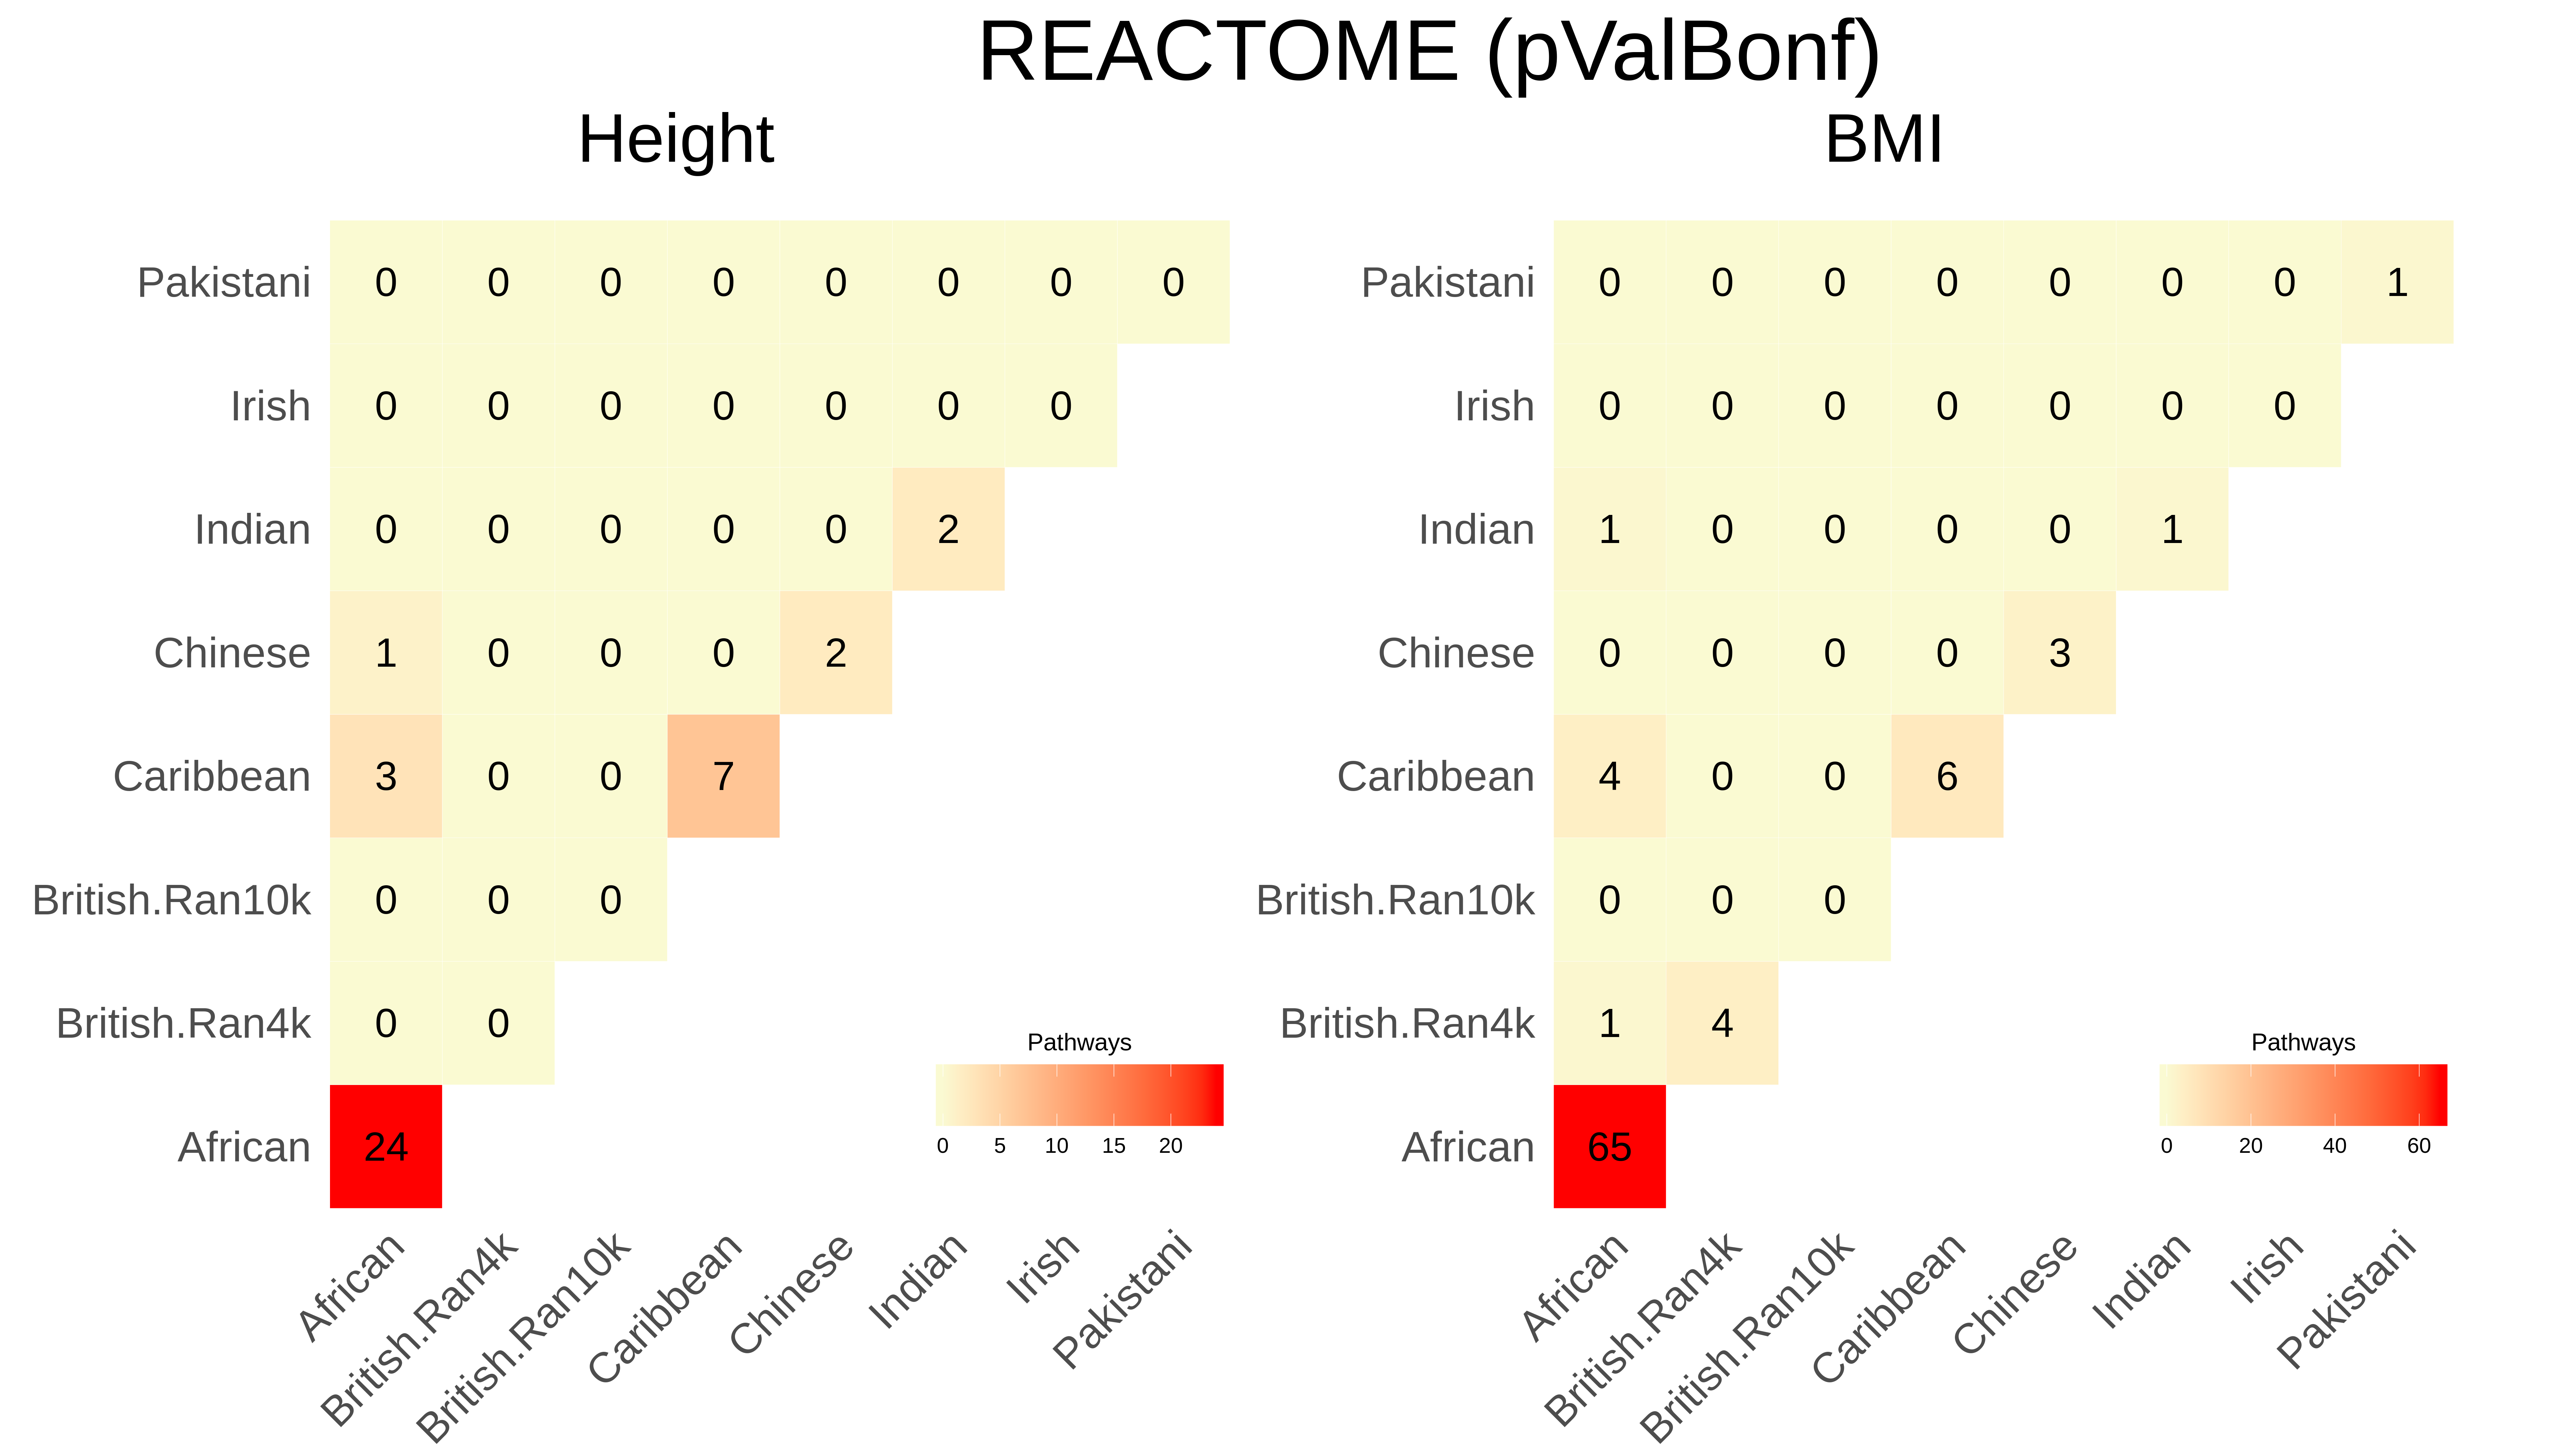
\includegraphics[scale=.225]{Images/Supp/InterPath_Supp_Figure_Heatplots_REACTOME_vs1.png}
\caption[TBD]{\textbf{TBD}. \\ See above (this would be a supplementary figure).}
\label{InterPath-Supp-Figure-Heatplots-REACTOME}
\end{figure}
\clearpage

%\begin{figure}[htbp]
%\centering
%\includegraphics[scale=.15]{Images/Main/InterPath_Main_PopCompDotPlots_African_vs1.png}
%\caption[]{\textbf{MAPIT-R Cross-Population KEGG $p$-value Comparisons: African}. Shown are comparisons of each population subset's MAPIT-R $p$-value for Height and BMI in KEGG against the African subset's MAPIT-R $p$-values. On the $x$-axis are the African subset's observed -$\log_{10}$ $p$-value and on the $y$-axis is the other population's observed -$\log_{10}$ $p$-value. Dotted red lines represent Bonferroni-corrected $p$-value thresholds for each population/phenotype combination.}
%\label{InterPath-Main-Figure-PopCompDotPlots}
%\end{figure}
%\clearpage

\begin{landscape}
\begin{figure}[htbp]
\centering
\hspace*{-.5cm}
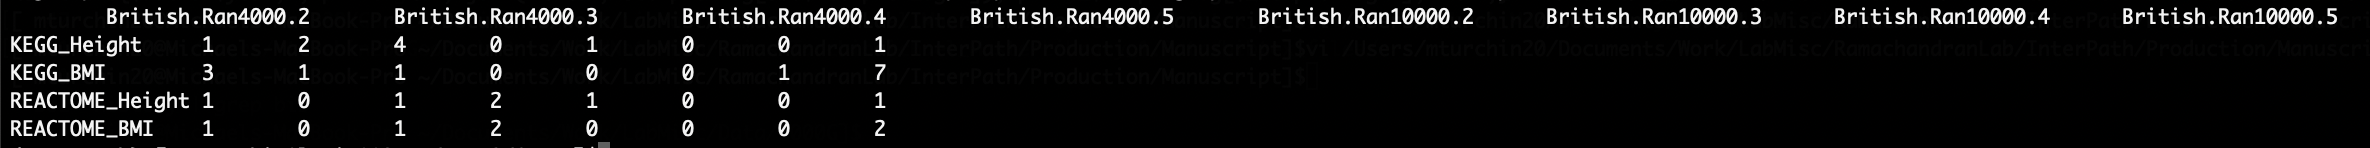
\includegraphics[scale=1]{Images/Supp/InterPath_Supp_Figure_BritReps_Barplot_Temp.png}
\caption[TBD]{\textbf{TBD}. }
\label{InterPath-Supp-Figure-BritReps-Barplots}
\end{figure}
\end{landscape}
\clearpage

%\begin{figure}[htbp]
%\centering
%\includegraphics[scale=.15]{Images/Supp/InterPath_Supp_Figure_PhenoCompDotPlots_vs1.png}
%\caption[TBD]{\textbf{MAPIT-R Phenotype $p$-value Comparisons}. \\ Shown is a comparison of the MAPIT-R $p$-values for both phenotypes analyzed across all population subsets in the KEGG database. Shown on the $x$-axis is the observed height -$\log_{10}$ MAPIT-R $p$-value and shown on the $y$-axis is the observed BMI -$\log_{10}$ MAPIT-R $p$-value. Dotted red lines represent Bonferroni-corrected $p$-value thresholds for each population/phenotype combination (.05 / number of KEGG pathways analyzed). In general we observe a correlation between MAPIT-R $p$-values between each phenotype. In the African subset, where we have the most observed power, we find pathways that are significant in both phenotypes as well as each phenotype separately. Additionally, we observe, among marginally significant pathways, stronger MAPIT-R signals in BMI than height -- this is in line with previous observations that BMI may contain higher levels of epistasis than height (citations).}
%\label{InterPath-Supp-Figure-PhenoCompDotPlots}
%\end{figure}
%\clearpage

\begin{figure}[htbp]
\centering
\includegraphics[scale=.15]{Images/Supp/InterPath_Supp_Figure_IBS_AllPops_vs2.png}
\caption[TBD]{\textbf{IBS Proportions vs. MAPIT-R $p$-values in All UKB Subsets}}
\label{InterPath-Supp-Figure-IBS-AllPops}
\end{figure}
\clearpage

\begin{figure}[htbp]
\centering
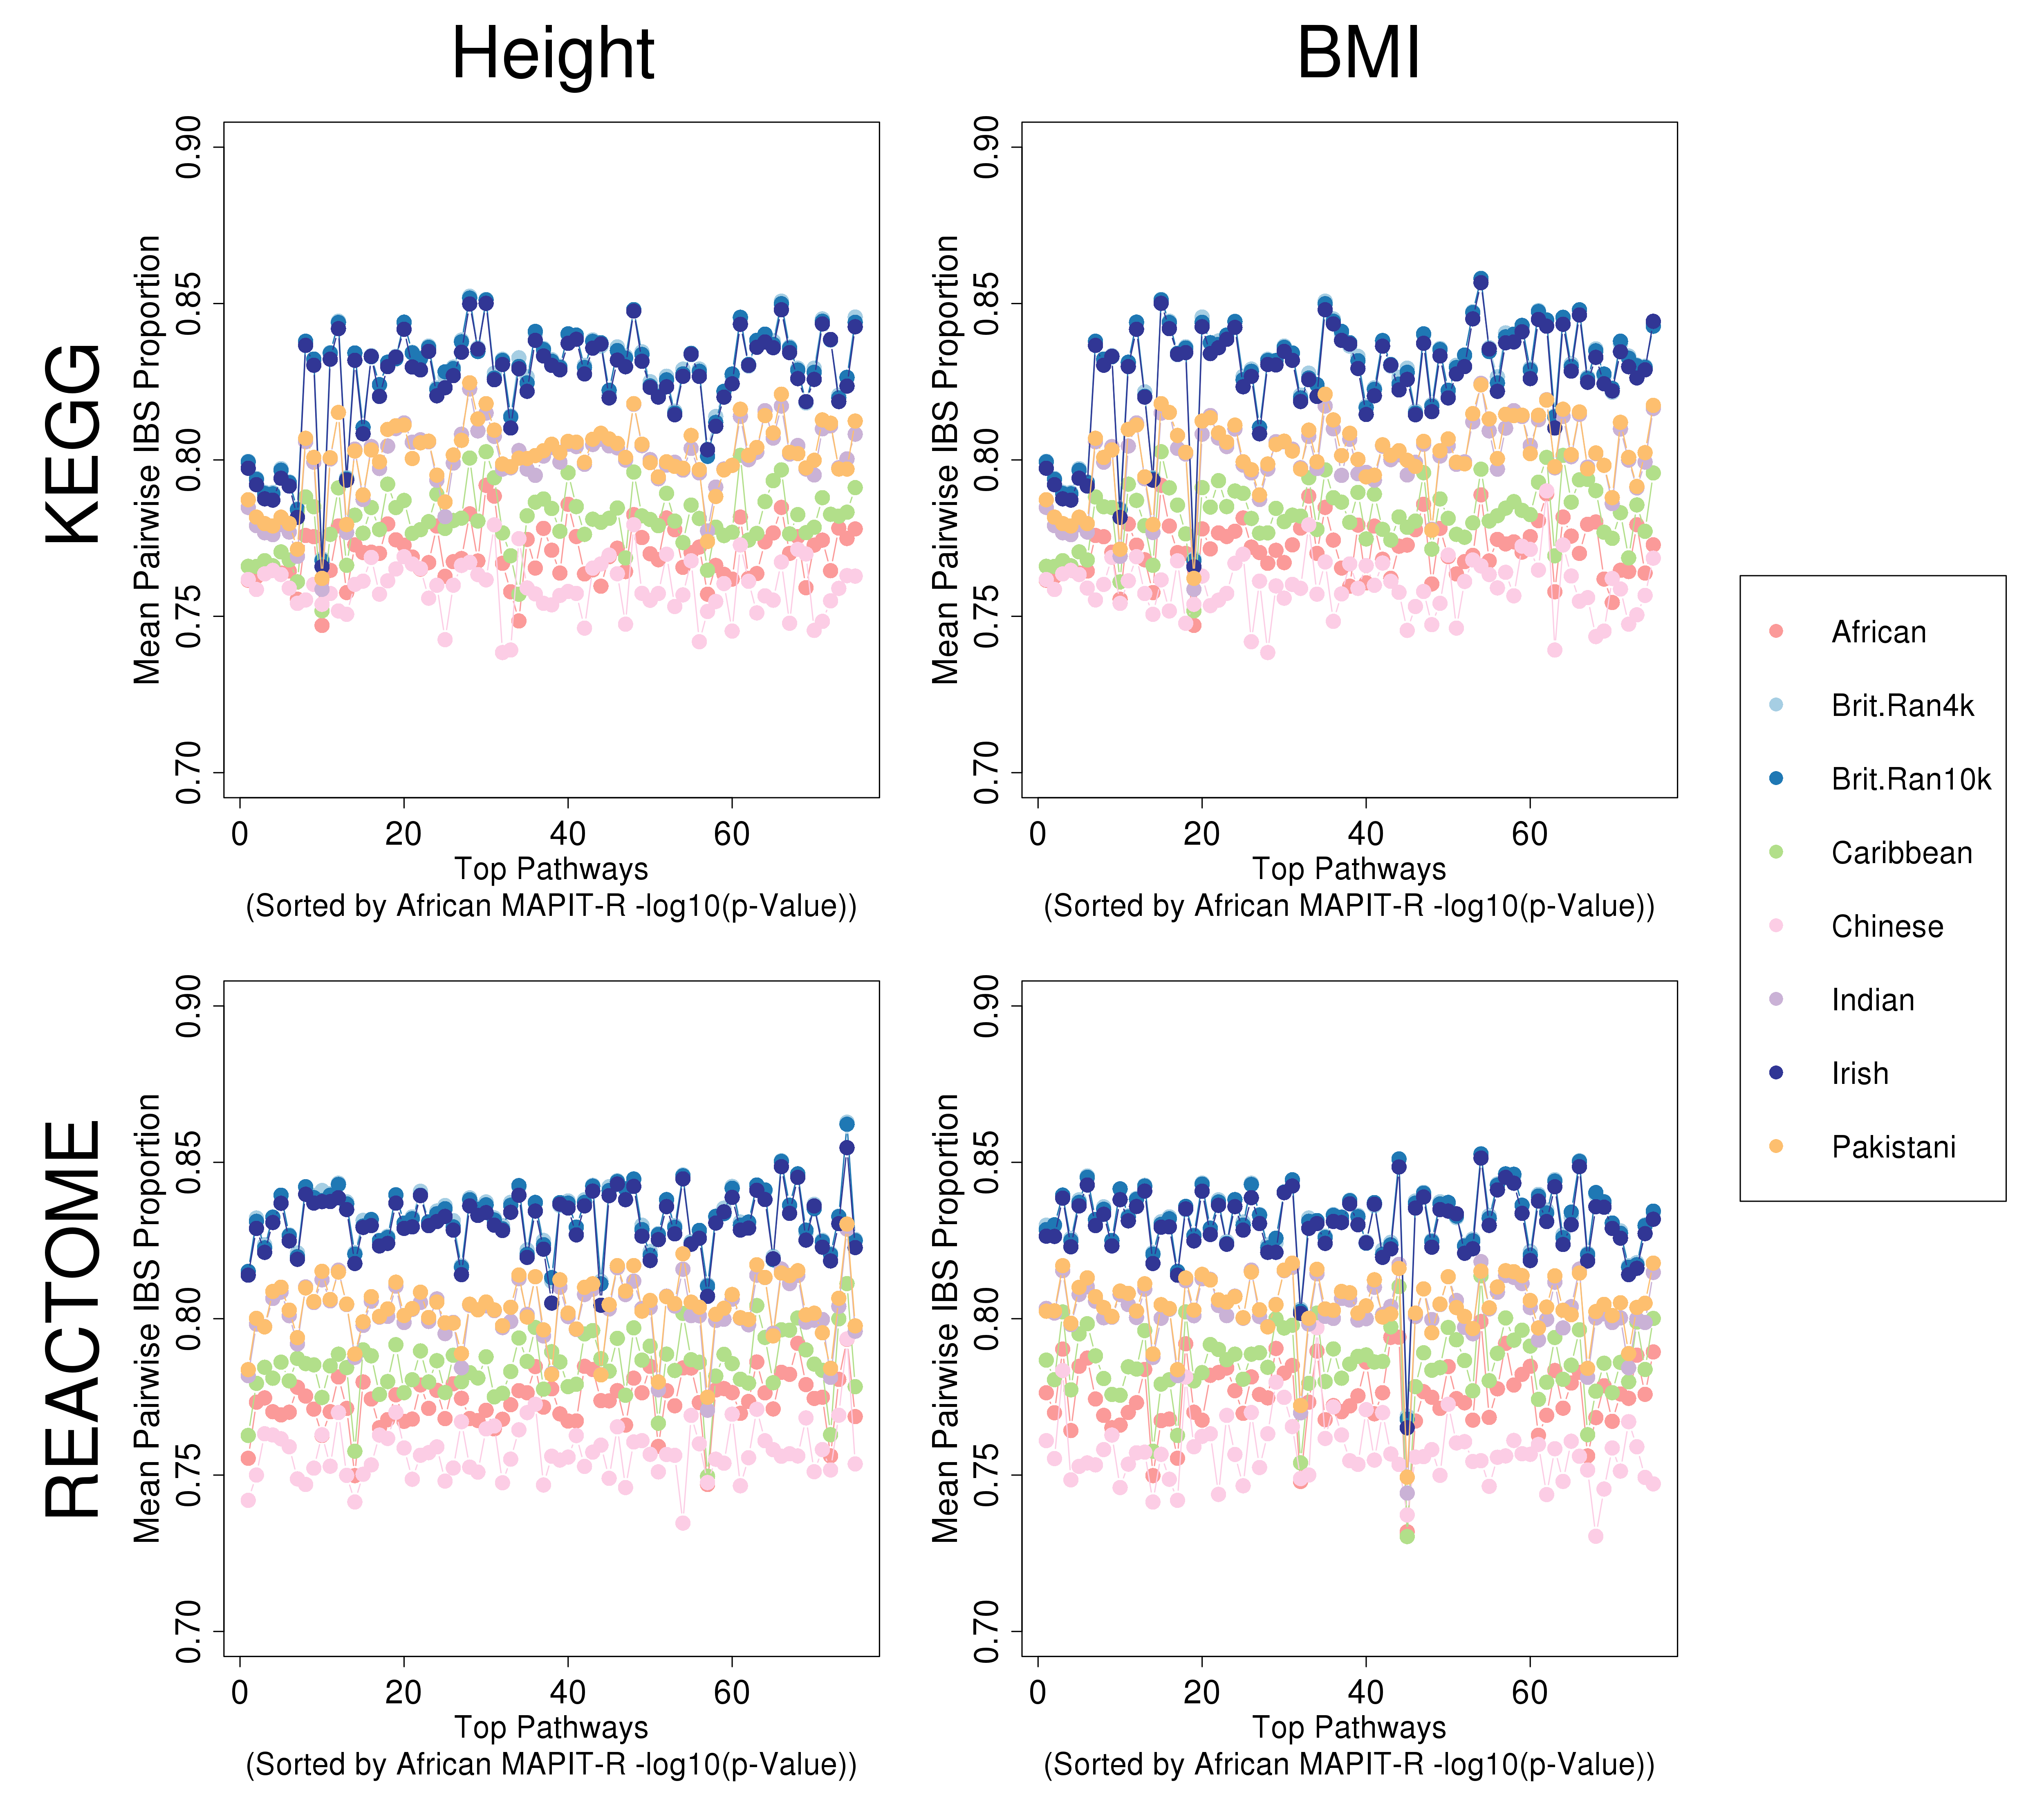
\includegraphics[scale=.35]{Images/Supp/InterPath_Supp_Figure_IBS_AllPopComps_vs2.png}
\caption[TBD]{\textbf{IBS in Top Pathways Across Populations}.}
\label{InterPath-Supp-Figure-IBS-AllPopComps}
\end{figure}
\clearpage

\section{Supplementary Tables}\label{Supplementary-Tables}

\begin{table}[ht]
\centering
\begin{tabular}{ccccc}
  \hline
\textbf{UK BioBank} & \textbf{Individuals} & \textbf{SNPs} & \textbf{KEGG} & \textbf{REACTOME} \\
\textbf{Subset} & & & \textbf{Pathways} & \textbf{Pathways}  \\
  \hline
\textbf{Original Subsets:} & & & & \\
African & 3111 & 374466 & 180 & 658 \\ 
British.Ran4000 & 3848 & 600006 & 173 & 650 \\ 
British.Ran10000 & 9603 & 597298 & 186 & 669 \\ 
Caribbean & 3833 & 410017 & 181 & 661 \\ 
Chinese & 1448 & 345221 & 153 & 626 \\ 
Indian & 5077 & 505854 & 181 & 662 \\ 
Irish & 11575 & 588324 & 186 & 671 \\ 
Pakistani & 1581 & 516806 & 141 & 596 \\ 
\\
\textbf{British Replicates:} & & & & \\
British.Ran4000.2 & 3869 & 599381 & 173 & 650 \\ 
British.Ran4000.3 & 3836 & 600654 & 173 & 649 \\ 
British.Ran4000.4 & 3838 & 599829 & 173 & 650 \\ 
British.Ran4000.5 & 3853 & 599442 & 173 & 650 \\ 
British.Ran10000.2 & 9628 & 597577 & 186 & 669 \\ 
British.Ran10000.3 & 9636 & 597486 & 186 & 669 \\ 
British.Ran10000.4 & 9593 & 597369 & 186 & 669 \\ 
British.Ran10000.5 & 9596 & 597507 & 186 & 669 \\ 
  \hline
\end{tabular}
\caption[TBD]{\textbf{UK BioBank Subset Statistics}. \\ }
\label{InterPath-Supp-Table-UKBPopStats}
\end{table}
\clearpage

%From: https://tex.stackexchange.com/questions/118606/numbering-tables-a1-a2-etc-in-latex & https://tex.stackexchange.com/questions/83689/next-subsequent-letter-in-the-alphabet
\newcounter{CharNumber1}
\setcounter{CharNumber1}{1}
\renewcommand{\thetable}{\arabic{table}\alph{CharNumber1}}
\begin{landscape}
\begin{table}[ht]
\centering
\vspace*{-.75cm}
\begin{tabular}{lccc}
  \hline
\textbf{Population \& Pathway} & \textbf{Genes} & \textbf{SNPs} & \textbf{p-Value} \\ 
  \hline
  \textbf{African:} & & & \\
 KEGG\_CHEMOKINE\_SIGNALING\_PATHWAY & 170 & 2448 & 5.136E-10 \\
 KEGG\_AXON\_GUIDANCE & 120 & 3045 & 1.511E-08 \\ 
  KEGG\_HYPERTROPHIC\_CARDIOMYOPATHY\_HCM & 77 & 2132 & 1.542E-08 \\ 
  KEGG\_CYTOKINE\_CYTOKINE\_RECEPTOR\_INTERACTION & 234 & 2279 & 2.837E-08 \\ 
  KEGG\_PURINE\_METABOLISM & 135 & 2411 & 1.186E-07 \\ 
  KEGG\_DILATED\_CARDIOMYOPATHY & 83 & 2234 & 1.242E-07 \\ 
  KEGG\_TYPE\_I\_DIABETES\_MELLITUS & 38 & 1659 & 1.330E-07 \\ 
  KEGG\_ENDOCYTOSIS & 169 & 2981 & 1.523E-07 \\ 
  KEGG\_OLFACTORY\_TRANSDUCTION & 365 & 3110 & 1.194E-06 \\ 
  KEGG\_AUTOIMMUNE\_THYROID\_DISEASE & 48 & 1504 & 1.492E-06 \\ 
  KEGG\_NATURAL\_KILLER\_CELL\_MEDIATED\_CYTOTOXICITY & 127 & 2216 & 5.160E-06 \\ 
  KEGG\_ALZHEIMERS\_DISEASE & 136 & 1846 & 5.188E-06 \\ 
  KEGG\_WNT\_SIGNALING\_PATHWAY & 141 & 2050 & 6.536E-06 \\ 
  KEGG\_ALLOGRAFT\_REJECTION & 32 & 1329 & 8.152E-06 \\ 
  KEGG\_HUNTINGTONS\_DISEASE & 148 & 1660 & 8.639E-06 \\ 
  KEGG\_GRAFT\_VERSUS\_HOST\_DISEASE & 35 & 1348 & 8.933E-06 \\ 
  KEGG\_GAP\_JUNCTION & 85 & 1851 & 9.300E-06 \\ 
  KEGG\_SYSTEMIC\_LUPUS\_ERYTHEMATOSUS & 111 & 1525 & 1.499E-05 \\ 
  KEGG\_VIRAL\_MYOCARDITIS & 64 & 1972 & 1.889E-05 \\ 
  KEGG\_ANTIGEN\_PROCESSING\_AND\_PRESENTATION & 74 & 1598 & 2.890E-05 \\ 
  KEGG\_LONG\_TERM\_POTENTIATION & 63 & 1585 & 3.317E-05 \\ 
  KEGG\_INTESTINAL\_IMMUNE\_NETWORK\_FOR\_IGA\_PRODUCTION & 43 & 1072 & 3.838E-05 \\ 
  KEGG\_PHOSPHATIDYLINOSITOL\_SIGNALING\_SYSTEM & 75 & 1681 & 4.497E-05 \\ 
  KEGG\_ARRHYTHMOGENIC\_RIGHT\_VENTRICULAR\_CARDIOMYOPATHY\_ARVC & 70 & 2373 & 5.289E-05 \\ 
  KEGG\_LONG\_TERM\_DEPRESSION & 66 & 1741 & 5.553E-05 \\ 
  KEGG\_GLIOMA & 64 & 974 & 5.649E-05 \\ 
  KEGG\_VASCULAR\_SMOOTH\_MUSCLE\_CONTRACTION & 106 & 2465 & 1.881E-04 \\ 
  KEGG\_REGULATION\_OF\_ACTIN\_CYTOSKELETON & 194 & 3047 & 1.951E-04 \\ 
  KEGG\_TYPE\_II\_DIABETES\_MELLITUS & 45 & 979 & 2.687E-04 \\ 
   \hline
\end{tabular}
\caption[TBD]{\textbf{Genome-Wide Significant MAPIT-R Pathways: KEGG Height}. \\ }
\label{InterPath-Supp-Table-TopPathways-KEGG-Height-a}
\end{table}
\addtocounter{table}{-1}
%\addtocounter{CharNumber1}{1}
\clearpage

\begin{table}[ht]
\centering
\vspace*{-.75cm}
\begin{tabular}{lccc}
  \hline
  \textbf{British.Ran4000:} & & & \\
  KEGG\_ERBB\_SIGNALING\_PATHWAY & 83 & 2674 & 1.003E-05 \\
KEGG\_TYPE\_I\_DIABETES\_MELLITUS &  39 & 1924 & 1.693E-05 \\ 
 \textcolor{white}{KEGG\_ARRHYTHMOGENIC\_RIGHT\_VENTRICULAR\_CARDIOMYOPATHY\_ARVC } & & & \\
 \textbf{Caribbean:} & & & \\
 KEGG\_CHEMOKINE\_SIGNALING\_PATHWAY & 171 & 2688 & 2.733E-06 \\
 KEGG\_NATURAL\_KILLER\_CELL\_MEDIATED\_CYTOTOXICITY & 128 & 2356 & 1.125E-05 \\
  KEGG\_CELL\_ADHESION\_MOLECULES\_CAMS & 120 & 4029 & 1.770E-05 \\
  KEGG\_LEUKOCYTE\_TRANSENDOTHELIAL\_MIGRATION & 105 & 1941 & 2.169E-05 \\
  KEGG\_VASCULAR\_SMOOTH\_MUSCLE\_CONTRACTION & 106 & 2708 & 3.675E-05 \\
  KEGG\_AXON\_GUIDANCE & 120 & 3365 & 1.088E-04 \\
  KEGG\_SMALL\_CELL\_LUNG\_CANCER & 78 & 1931 & 1.369E-04 \\
  KEGG\_ARRHYTHMOGENIC\_RIGHT\_VENTRICULAR\_CARDIOMYOPATHY\_ARVC & 70 & 2581 & 1.376E-04 \\
  KEGG\_HYPERTROPHIC\_CARDIOMYOPATHY\_HCM & 77 & 2298 & 1.960E-04 \\
 \\
 \textbf{Chinese:} & & & \\
 KEGG\_TYPE\_I\_DIABETES\_MELLITUS & 39 & 1573 & 1.269E-08 \\
 KEGG\_ANTIGEN\_PROCESSING\_AND\_PRESENTATION & 75 & 1505 & 8.287E-08 \\
  KEGG\_MELANOGENESIS & 96 & 1382 & 1.028E-05 \\
  KEGG\_ALLOGRAFT\_REJECTION & 33 & 1250 & 1.183E-05 \\
  KEGG\_GRAFT\_VERSUS\_HOST\_DISEASE & 37 & 1274 & 2.424E-05 \\
  KEGG\_NON\_SMALL\_CELL\_LUNG\_CANCER & 53 & 1081 & 5.337E-05 \\
  KEGG\_SYSTEMIC\_LUPUS\_ERYTHEMATOSUS & 109 & 1399 & 1.252E-04 \\
 \\
 \textbf{Indian:} & & & \\
 KEGG\_NON\_SMALL\_CELL\_LUNG\_CANCER & 53 & 1696 & 4.182E-05 \\
 KEGG\_CYTOKINE\_CYTOKINE\_RECEPTOR\_INTERACTION & 237 & 2995 & 4.965E-05 \\
  KEGG\_REGULATION\_OF\_ACTIN\_CYTOSKELETON & 193 & 4069 & 1.963E-04 \\
  KEGG\_ERBB\_SIGNALING\_PATHWAY & 83 & 2174 & 2.128E-04 \\
   \hline
\end{tabular}
\caption[TBD]{\textbf{Genome-Wide Significant MAPIT-R Pathways: KEGG Height}. Continued. \\ }
\label{InterPath-Supp-Table-TopPathways-KEGG-Height-b}
\end{table}
\addtocounter{table}{-1}
%\addtocounter{CharNumber1}{1}

\begin{table}[ht]
\centering
\vspace*{-.75cm}
\begin{tabular}{lccc}
  \hline
 \textbf{Pakistani:} & & & \\
 KEGG\_ANTIGEN\_PROCESSING\_AND\_PRESENTATION & 78 & 1775 & 1.581E-08 \\
 KEGG\_AMINO\_SUGAR\_AND\_NUCLEOTIDE\_SUGAR\_METABOLISM & 40 & 610 & 7.840E-05 \\
  KEGG\_AUTOIMMUNE\_THYROID\_DISEASE & 49 & 1680 & 2.602E-04 \\
 \\
   \hline
\end{tabular}
\caption[TBD]{\textbf{Genome-Wide Significant MAPIT-R Pathways: KEGG Height}. Continued. \\ }
\label{InterPath-Supp-Table-TopPathways-KEGG-Height-c}
\end{table}
\addtocounter{table}{-1}
\addtocounter{CharNumber1}{1}
\clearpage

\begin{table}[ht]
\centering
\vspace*{-.75cm}
\begin{tabular}{lccc}
  \hline
\textbf{Population \& Pathway} & \textbf{Genes} & \textbf{SNPs} & \textbf{p-Value} \\ 
  \hline
  \textbf{African:} & & & \\
  KEGG\_AXON\_GUIDANCE & 120 & 3045 & 0.000E+00 \\
 KEGG\_SMALL\_CELL\_LUNG\_CANCER & 78 & 1776 & 3.199E-10 \\
  KEGG\_TYPE\_I\_DIABETES\_MELLITUS & 38 & 1659 & 4.291E-10 \\
  KEGG\_REGULATION\_OF\_ACTIN\_CYTOSKELETON & 194 & 3047 & 8.253E-10 \\
  KEGG\_AUTOIMMUNE\_THYROID\_DISEASE & 48 & 1504 & 1.393E-08 \\
  KEGG\_CHEMOKINE\_SIGNALING\_PATHWAY & 170 & 2448 & 1.512E-08 \\
  KEGG\_ALLOGRAFT\_REJECTION & 32 & 1329 & 2.529E-08 \\
  KEGG\_GRAFT\_VERSUS\_HOST\_DISEASE & 35 & 1348 & 4.753E-08 \\
  KEGG\_NATURAL\_KILLER\_CELL\_MEDIATED\_CYTOTOXICITY & 127 & 2216 & 1.081E-07 \\
  KEGG\_WNT\_SIGNALING\_PATHWAY & 141 & 2050 & 1.414E-07 \\
  KEGG\_SYSTEMIC\_LUPUS\_ERYTHEMATOSUS & 111 & 1525 & 1.504E-07 \\
  KEGG\_HYPERTROPHIC\_CARDIOMYOPATHY\_HCM & 77 & 2132 & 1.578E-07 \\
  KEGG\_ANTIGEN\_PROCESSING\_AND\_PRESENTATION & 74 & 1598 & 2.075E-07 \\
  KEGG\_ERBB\_SIGNALING\_PATHWAY & 83 & 1538 & 3.298E-07 \\
  KEGG\_OLFACTORY\_TRANSDUCTION & 365 & 3110 & 8.627E-07 \\
  KEGG\_GAP\_JUNCTION & 85 & 1851 & 8.996E-07 \\
  KEGG\_VIRAL\_MYOCARDITIS & 64 & 1972 & 1.086E-06 \\
  KEGG\_ARRHYTHMOGENIC\_RIGHT\_VENTRICULAR\_CARDIOMYOPATHY\_ARVC & 70 & 2373 & 1.581E-06 \\
  KEGG\_NON\_SMALL\_CELL\_LUNG\_CANCER & 53 & 1243 & 1.640E-06 \\
  KEGG\_JAK\_STAT\_SIGNALING\_PATHWAY & 138 & 1324 & 2.000E-06 \\
  KEGG\_PURINE\_METABOLISM & 135 & 2411 & 2.463E-06 \\
  KEGG\_GLIOMA & 64 & 974 & 3.564E-06 \\
  KEGG\_T\_CELL\_RECEPTOR\_SIGNALING\_PATHWAY & 102 & 1373 & 6.120E-06 \\
  KEGG\_DILATED\_CARDIOMYOPATHY & 83 & 2234 & 6.987E-06 \\
  KEGG\_ENDOCYTOSIS & 169 & 2981 & 8.023E-06 \\
  KEGG\_ALZHEIMERS\_DISEASE & 136 & 1846 & 8.567E-06 \\
  KEGG\_TYPE\_II\_DIABETES\_MELLITUS & 45 & 979 & 8.598E-06 \\
  KEGG\_HUNTINGTONS\_DISEASE & 148 & 1660 & 1.310E-05 \\
  KEGG\_VALINE\_LEUCINE\_AND\_ISOLEUCINE\_DEGRADATION & 41 & 399 & 1.710E-05 \\
   \hline
\end{tabular}
\caption[TBD]{\textbf{Genome-Wide Significant MAPIT-R Pathways: KEGG BMI}. \\ }
\label{InterPath-Supp-Table-TopPathways-KEGG-BMI-a}
\end{table}
\addtocounter{table}{-1}
%\addtocounter{CharNumber1}{1}

\begin{table}[ht]
\centering
\vspace*{-.75cm}
\begin{tabular}{lccc}
  \hline
  KEGG\_ADHERENS\_JUNCTION & 66 & 1603 & 2.023E-05 \\
  KEGG\_VASCULAR\_SMOOTH\_MUSCLE\_CONTRACTION & 106 & 2465 & 2.410E-05 \\
  KEGG\_LONG\_TERM\_POTENTIATION & 63 & 1585 & 2.624E-05 \\
  KEGG\_INTESTINAL\_IMMUNE\_NETWORK\_FOR\_IGA\_PRODUCTION & 43 & 1072 & 2.987E-05 \\
  KEGG\_P53\_SIGNALING\_PATHWAY & 63 & 527 & 3.529E-05 \\
  KEGG\_NEUROTROPHIN\_SIGNALING\_PATHWAY & 117 & 1483 & 7.897E-05 \\
  KEGG\_BETA\_ALANINE\_METABOLISM & 20 & 295 & 1.127E-04 \\
  KEGG\_ECM\_RECEPTOR\_INTERACTION & 81 & 2116 & 1.185E-04 \\
  KEGG\_ETHER\_LIPID\_METABOLISM & 28 & 337 & 1.406E-04 \\
  KEGG\_LEISHMANIA\_INFECTION & 64 & 1353 & 1.441E-04 \\
  KEGG\_CELL\_CYCLE & 115 & 858 & 1.484E-04 \\
  KEGG\_INOSITOL\_PHOSPHATE\_METABOLISM & 53 & 849 & 1.534E-04 \\
  KEGG\_LEUKOCYTE\_TRANSENDOTHELIAL\_MIGRATION & 105 & 1786 & 1.633E-04 \\
  KEGG\_HOMOLOGOUS\_RECOMBINATION & 22 & 248 & 1.749E-04 \\
  KEGG\_O\_GLYCAN\_BIOSYNTHESIS & 25 & 575 & 1.923E-04 \\
  KEGG\_MELANOGENESIS & 98 & 1516 & 1.971E-04 \\
  KEGG\_ASTHMA & 26 & 850 & 2.636E-04 \\
  KEGG\_PROSTATE\_CANCER & 85 & 1143 & 2.640E-04 \\
  \\
  \textbf{British.Ran4000:} & & & \\
  KEGG\_NATURAL\_KILLER\_CELL\_MEDIATED\_CYTOTOXICITY & 128 & 3133 & 2.205E-06 \\
  KEGG\_TYPE\_I\_DIABETES\_MELLITUS & 39 & 1924 & 2.335E-05 \\
  KEGG\_ANTIGEN\_PROCESSING\_AND\_PRESENTATION & 79 & 1728 & 3.659E-05 \\
  KEGG\_JAK\_STAT\_SIGNALING\_PATHWAY & 139 & 2076 & 1.139E-04 \\
 \textcolor{white}{KEGG\_ARRHYTHMOGENIC\_RIGHT\_VENTRICULAR\_CARDIOMYOPATHY\_ARVC } & & & \\
 \textbf{Caribbean:} & & & \\
 KEGG\_CHEMOKINE\_SIGNALING\_PATHWAY & 171 & 2688 & 1.086E-06 \\
 KEGG\_CYTOKINE\_CYTOKINE\_RECEPTOR\_INTERACTION & 237 & 2453 & 4.294E-06 \\
  KEGG\_ARRHYTHMOGENIC\_RIGHT\_VENTRICULAR\_CARDIOMYOPATHY\_ARVC & 70 & 2581 & 2.070E-05 \\
   KEGG\_AXON\_GUIDANCE & 120 & 3365 & 2.382E-05 \\
  KEGG\_OLFACTORY\_TRANSDUCTION & 366 & 3318 & 5.058E-05 \\
   \hline
\end{tabular}
\caption[TBD]{\textbf{Genome-Wide Significant MAPIT-R Pathways: KEGG BMI}. Continued. \\ }
\label{InterPath-Supp-Table-TopPathways-KEGG-BMI-b}
\end{table}
\addtocounter{table}{-1}
%\addtocounter{CharNumber1}{1}

\begin{table}[ht]
\centering
\vspace*{-.75cm}
\begin{tabular}{lccc}
  \hline
  KEGG\_REGULATION\_OF\_ACTIN\_CYTOSKELETON & 193 & 3340 & 9.265E-05 \\
  KEGG\_VASCULAR\_SMOOTH\_MUSCLE\_CONTRACTION & 106 & 2708 & 1.374E-04 \\
  \\
 \textbf{Chinese:} & & & \\
 KEGG\_ANTIGEN\_PROCESSING\_AND\_PRESENTATION & 75 & 1505 & 4.430E-09 \\
 KEGG\_SYSTEMIC\_LUPUS\_ERYTHEMATOSUS & 109 & 1399 & 4.766E-07 \\
  KEGG\_LEISHMANIA\_INFECTION & 65 & 1263 & 1.224E-06 \\
  KEGG\_VIRAL\_MYOCARDITIS & 65 & 1808 & 2.157E-06 \\
  KEGG\_ALLOGRAFT\_REJECTION & 33 & 1250 & 2.648E-05 \\
  KEGG\_FC\_EPSILON\_RI\_SIGNALING\_PATHWAY & 76 & 1241 & 4.929E-05 \\
  KEGG\_TYPE\_I\_DIABETES\_MELLITUS & 39 & 1573 & 7.376E-05 \\
  KEGG\_GRAFT\_VERSUS\_HOST\_DISEASE & 37 & 1274 & 1.049E-04 \\
  \textcolor{white}{KEGG\_ARRHYTHMOGENIC\_RIGHT\_VENTRICULAR\_CARDIOMYOPATHY\_ARVC } & & & \\
 \textbf{Indian:} & & & \\
 KEGG\_ENDOCYTOSIS & 170 & 4003 & 8.651E-09 \\
 KEGG\_CYTOKINE\_CYTOKINE\_RECEPTOR\_INTERACTION & 237 & 2995 & 9.500E-05 \\
  KEGG\_REGULATION\_OF\_ACTIN\_CYTOSKELETON & 193 & 4069 & 1.034E-04 \\
  KEGG\_ERBB\_SIGNALING\_PATHWAY & 83 & 2174 & 1.827E-04 \\
 \\
 \textbf{Pakistani:} & & & \\
 KEGG\_GRAFT\_VERSUS\_HOST\_DISEASE & 37 & 1466 & 5.412E-06 \\
 KEGG\_ANTIGEN\_PROCESSING\_AND\_PRESENTATION & 78 & 1775 & 6.724E-06 \\
  KEGG\_ALLOGRAFT\_REJECTION & 33 & 1442 & 1.214E-05 \\
  KEGG\_AUTOIMMUNE\_THYROID\_DISEASE & 49 & 1680 & 1.978E-05 \\
  KEGG\_MELANOMA & 68 & 1352 & 8.436E-05 \\
 \\
   \hline
\end{tabular}
\caption[TBD]{\textbf{Genome-Wide Significant MAPIT-R Pathways: KEGG BMI}. Continued. \\ }
\label{InterPath-Supp-Table-TopPathways-KEGG-BMI-c}
\end{table}
\addtocounter{table}{-1}
\addtocounter{CharNumber1}{1}
\clearpage

\begin{table}[ht]
\centering
\vspace*{-.75cm}
\begin{tabular}{lccc}
  \hline
\textbf{Population \& Pathway} & \textbf{Genes} & \textbf{SNPs} & \textbf{p-Value} \\ 
  \hline
  \textbf{African:} & & & \\
  REACTOME\_GASTRIN\_CREB\_SIGNALLING\_PATHWAY\_VIA\_PKC\_AND\_MAPK & 183 & 2980 & 4.861E-10 \\
  REACTOME\_NEUROTRANSMITTER\_RECEPTOR\_BINDING\_AND\_DOWNSTREAM\_ & 125 & 2942 & 3.431E-09 \\
  \qquad TRANSMISSION\_IN\_THE\_POSTSYNAPTIC\_CELL & & & \\
  REACTOME\_SIGNALING\_BY\_RHO\_GTPASES & 96 & 2385 & 6.821E-09 \\
  REACTOME\_CLASS\_A1\_RHODOPSIN\_LIKE\_RECEPTORS & 261 & 2502 & 3.245E-08 \\
  REACTOME\_TRANSPORT\_OF\_INORGANIC\_CATIONS\_ANIONS\_AND\_AMINO\_ & 86 & 1511 & 6.637E-08 \\
  \qquad ACIDS\_OLIGOPEPTIDES & & & \\
  REACTOME\_CYTOKINE\_SIGNALING\_IN\_IMMUNE\_SYSTEM & 253 & 3100 & 8.416E-08 \\
  REACTOME\_INNATE\_IMMUNE\_SYSTEM & 236 & 2334 & 1.464E-07 \\
  REACTOME\_L1CAM\_INTERACTIONS & 73 & 1679 & 7.396E-07 \\
  REACTOME\_G\_ALPHA\_Q\_SIGNALLING\_EVENTS & 164 & 2636 & 8.124E-07 \\
  REACTOME\_CELL\_CYCLE & 351 & 2459 & 1.275E-06 \\
  REACTOME\_CELL\_CELL\_COMMUNICATION & 107 & 3031 & 1.685E-06 \\
  REACTOME\_HEPARAN\_SULFATE\_HEPARIN\_HS\_GAG\_METABOLISM & 43 & 1170 & 2.873E-06 \\
  REACTOME\_INTEGRIN\_CELL\_SURFACE\_INTERACTIONS & 76 & 1594 & 4.270E-06 \\
  REACTOME\_PHOSPHOLIPID\_METABOLISM & 175 & 2260 & 7.533E-06 \\
  REACTOME\_MHC\_CLASS\_II\_ANTIGEN\_PRESENTATION & 81 & 1215 & 7.852E-06 \\
  REACTOME\_SIGNALING\_BY\_PDGF & 115 & 1902 & 9.120E-06 \\
  REACTOME\_PLATELET\_HOMEOSTASIS & 71 & 1453 & 9.317E-06 \\
  REACTOME\_SIGNALING\_BY\_NOTCH & 89 & 1534 & 1.695E-05 \\
  REACTOME\_METABOLISM\_OF\_CARBOHYDRATES & 207 & 2990 & 2.512E-05 \\
  REACTOME\_SEMAPHORIN\_INTERACTIONS & 62 & 1074 & 4.253E-05 \\
  REACTOME\_TRANSPORT\_OF\_GLUCOSE\_AND\_OTHER\_SUGARS\_BILE\_SALTS\_ & 87 & 1190 & 4.679E-05 \\
  \qquad AND\_ORGANIC\_ACIDS\_METAL\_IONS\_AND\_AMINE\_COMPOUNDS & & & \\
  REACTOME\_SIGNALING\_BY\_ERBB4 & 85 & 1483 & 4.911E-05 \\
  REACTOME\_OPIOID\_SIGNALLING & 71 & 1467 & 5.233E-05 \\
  REACTOME\_CELL\_JUNCTION\_ORGANIZATION & 67 & 1701 & 7.339E-05 \\
  \\
   \textbf{British.Ran4000:} & & & \\
  NA & & & \\
   \hline
\end{tabular}
\caption[TBD]{\textbf{Genome-Wide Significant MAPIT-R Pathways: REACTOME Height}. Continued. \\ }
\label{InterPath-Supp-Table-TopPathways-REACTOME-Height-a}
\end{table}
\addtocounter{table}{-1}
%\addtocounter{CharNumber1}{1}

\begin{table}[ht]
\centering
\vspace*{-.75cm}
\begin{tabular}{lccc}
  \hline
 \textbf{Caribbean:} & \textcolor{white}{Genes} & & \\
 REACTOME\_CLASS\_A1\_RHODOPSIN\_LIKE\_RECEPTORS & 263 & 2699 & 1.853E-07 \\
 REACTOME\_METABOLISM\_OF\_CARBOHYDRATES & 206 & 3283 & 7.116E-06 \\
  REACTOME\_SIGNALING\_BY\_RHO\_GTPASES & 97 & 2635 & 9.553E-06 \\
  REACTOME\_INTEGRATION\_OF\_ENERGY\_METABOLISM & 107 & 2158 & 1.004E-05 \\
  REACTOME\_GLYCOSAMINOGLYCAN\_METABOLISM & 97 & 2301 & 1.703E-05 \\
  REACTOME\_FACTORS\_INVOLVED\_IN\_MEGAKARYOCYTE\_DEVELOPMENT\_AND\_ & 118 & 1715 & 2.724E-05 \\
  \qquad PLATELET\_PRODUCTION & & & \\
  REACTOME\_PLATELET\_ACTIVATION\_SIGNALING\_AND\_AGGREGATION & 183 & 3354 & 5.992E-05 \\
  \textcolor{white}{REACTOME\_NEUROTRANSMITTER\_RECEPTOR\_BINDING\_AND\_DOWNSTREAM\_} & & & \\
 \textbf{Chinese:} & & & \\
 REACTOME\_MHC\_CLASS\_II\_ANTIGEN\_PRESENTATION & 82 & 1118 & 1.861E-06 \\
 REACTOME\_INTERFERON\_GAMMA\_SIGNALING & 59 & 1263 & 1.127E-05 \\
 \\
 \textbf{Indian:} & & & \\
 REACTOME\_SIGNALING\_BY\_EGFR\_IN\_CANCER & 102 & 2196 & 7.705E-06 \\
 REACTOME\_SIGNALING\_BY\_FGFR\_IN\_DISEASE & 120 & 2307 & 3.131E-05 \\
 \\
 \textbf{Pakistani:} & & & \\
 NA & & & \\
 \\
   \hline
\end{tabular}
\caption[TBD]{\textbf{Genome-Wide Significant MAPIT-R Pathways: REACTOME Height}. Continued. \\ }
\label{InterPath-Supp-Table-TopPathways-REACTOME-Height-b}
\end{table}
\addtocounter{table}{-1}
\addtocounter{CharNumber1}{1}
\clearpage

\begin{table}[ht]
\centering
\vspace*{-.75cm}
\begin{tabular}{lccc}
  \hline
\textbf{Population \& Pathway} & \textbf{Genes} & \textbf{SNPs} & \textbf{p-Value} \\ 
  \hline
  \textbf{African:} & & & \\
  REACTOME\_CYTOKINE\_SIGNALING\_IN\_IMMUNE\_SYSTEM & 253 & 3100 & 0.000E+00 \\
  REACTOME\_GASTRIN\_CREB\_SIGNALLING\_PATHWAY\_VIA\_PKC\_AND\_MAPK & 183 & 2980 & 0.000E+00 \\
  REACTOME\_G\_ALPHA\_Q\_SIGNALLING\_EVENTS & 164 & 2636 & 8.225E-09 \\
  REACTOME\_SIGNALING\_BY\_RHO\_GTPASES & 96 & 2385 & 3.098E-08 \\
  REACTOME\_INNATE\_IMMUNE\_SYSTEM & 236 & 2334 & 4.412E-08 \\
  REACTOME\_SIGNALING\_BY\_NOTCH & 89 & 1534 & 6.911E-08 \\
  REACTOME\_GLYCEROPHOSPHOLIPID\_BIOSYNTHESIS & 73 & 897 & 9.695E-08 \\
  REACTOME\_PHOSPHOLIPID\_METABOLISM & 175 & 2260 & 1.037E-07 \\
  REACTOME\_NGF\_SIGNALLING\_VIA\_TRKA\_FROM\_THE\_PLASMA\_MEMBRANE & 128 & 1957 & 1.412E-07 \\
  REACTOME\_CLASS\_B\_2\_SECRETIN\_FAMILY\_RECEPTORS & 75 & 864 & 1.758E-07 \\
  REACTOME\_SIGNALING\_BY\_PDGF & 115 & 1902 & 4.269E-07 \\
  REACTOME\_HEPARAN\_SULFATE\_HEPARIN\_HS\_GAG\_METABOLISM & 43 & 1170 & 7.242E-07 \\
  REACTOME\_HIV\_INFECTION & 171 & 1346 & 7.528E-07 \\
  REACTOME\_P75\_NTR\_RECEPTOR\_MEDIATED\_SIGNALLING & 67 & 1273 & 7.929E-07 \\
  REACTOME\_G\_ALPHA1213\_SIGNALLING\_EVENTS & 66 & 1382 & 8.905E-07 \\
  REACTOME\_SIGNALING\_BY\_ERBB2 & 95 & 1639 & 1.093E-06 \\
  REACTOME\_CELL\_CYCLE & 351 & 2459 & 1.288E-06 \\
  REACTOME\_OPIOID\_SIGNALLING & 71 & 1467 & 1.549E-06 \\
  REACTOME\_MEIOSIS & 92 & 659 & 2.306E-06 \\
  REACTOME\_CHONDROITIN\_SULFATE\_DERMATAN\_SULFATE\_METABOLISM & 41 & 1049 & 2.342E-06 \\
  REACTOME\_CELL\_CELL\_COMMUNICATION & 107 & 3031 & 2.783E-06 \\
  REACTOME\_M\_G1\_TRANSITION & 73 & 458 & 3.191E-06 \\
  REACTOME\_CLASS\_A1\_RHODOPSIN\_LIKE\_RECEPTORS & 261 & 2502 & 3.378E-06 \\
  REACTOME\_G\_ALPHA\_S\_SIGNALLING\_EVENTS & 110 & 1827 & 3.446E-06 \\
  REACTOME\_CELL\_JUNCTION\_ORGANIZATION & 67 & 1701 & 4.237E-06 \\
  REACTOME\_SIGNALING\_BY\_NOTCH1 & 61 & 1165 & 4.826E-06 \\
  REACTOME\_CELL\_CYCLE\_CHECKPOINTS & 105 & 670 & 5.781E-06 \\
  REACTOME\_PLC\_BETA\_MEDIATED\_EVENTS & 40 & 916 & 7.257E-06 \\
  REACTOME\_HOST\_INTERACTIONS\_OF\_HIV\_FACTORS & 112 & 963 & 7.521E-06 \\
   REACTOME\_NCAM1\_INTERACTIONS & 37 & 957 & 8.383E-06 \\
   \hline
\end{tabular}
\caption[TBD]{\textbf{Genome-Wide Significant MAPIT-R Pathways: REACTOME BMI}. \\ }
\label{InterPath-Supp-Table-TopPathways-REACTOME-BMI-a}
\end{table}
\addtocounter{table}{-1}
%\addtocounter{CharNumber1}{1}

\begin{table}[ht]
\centering
\vspace*{-.75cm}
\begin{tabular}{lccc}
  \hline
  REACTOME\_CD28\_CO\_STIMULATION & 31 & 421 & 8.809E-06 \\
  REACTOME\_GLYCOSAMINOGLYCAN\_METABOLISM & 97 & 2092 & 1.006E-05 \\
  REACTOME\_REGULATION\_OF\_INSULIN\_SECRETION & 81 & 1544 & 1.131E-05 \\
  REACTOME\_DOWNSTREAM\_SIGNALING\_EVENTS\_OF\_B\_CELL\_RECEPTOR\_BCR & 89 & 745 & 1.195E-05 \\
  REACTOME\_REGULATION\_OF\_APOPTOSIS & 52 & 564 & 1.218E-05 \\
  REACTOME\_FACTORS\_INVOLVED\_IN\_MEGAKARYOCYTE\_DEVELOPMENT\_AND\_ & 118 & 1560 & 1.264E-05 \\
  \qquad PLATELET\_PRODUCTION & \textcolor{white}{Genes} & & \\
  REACTOME\_MITOTIC\_G1\_G1\_S\_PHASES & 121 & 747 & 1.453E-05 \\
REACTOME\_NCAM\_SIGNALING\_FOR\_NEURITE\_OUT\_GROWTH & 61 & 1271 & 1.473E-05 \\
  REACTOME\_COSTIMULATION\_BY\_THE\_CD28\_FAMILY & 60 & 1005 & 1.745E-05 \\
  REACTOME\_ACTIVATION\_OF\_NF\_KAPPAB\_IN\_B\_CELLS & 59 & 465 & 1.861E-05 \\
  REACTOME\_HS\_GAG\_BIOSYNTHESIS & 25 & 932 & 1.901E-05 \\
  REACTOME\_MHC\_CLASS\_II\_ANTIGEN\_PRESENTATION & 81 & 1215 & 1.971E-05 \\
  REACTOME\_DOWNSTREAM\_SIGNAL\_TRANSDUCTION & 89 & 1288 & 1.980E-05 \\
  REACTOME\_MEIOTIC\_SYNAPSIS & 58 & 460 & 2.081E-05 \\
  REACTOME\_SIGNALING\_BY\_EGFR\_IN\_CANCER & 102 & 1579 & 2.106E-05 \\
  REACTOME\_POST\_NMDA\_RECEPTOR\_ACTIVATION\_EVENTS & 31 & 727 & 2.296E-05 \\
  REACTOME\_SIGNALING\_BY\_SCF\_KIT & 74 & 773 & 2.350E-05 \\
  REACTOME\_METABOLISM\_OF\_CARBOHYDRATES & 207 & 2990 & 3.003E-05 \\
  REACTOME\_HYALURONAN\_METABOLISM & 14 & 178 & 3.106E-05 \\
  REACTOME\_ASSEMBLY\_OF\_THE\_PRE\_REPLICATIVE\_COMPLEX & 60 & 331 & 3.293E-05 \\
  REACTOME\_ANTIGEN\_PROCESSING\_CROSS\_PRESENTATION & 68 & 850 & 3.956E-05 \\
  REACTOME\_NEUROTRANSMITTER\_RELEASE\_CYCLE & 30 & 631 & 4.501E-05 \\
  REACTOME\_CELL\_CYCLE\_MITOTIC & 274 & 1906 & 4.509E-05 \\
  REACTOME\_A\_TETRASACCHARIDE\_LINKER\_SEQUENCE\_IS\_REQUIRED\_FOR\_ & 21 & 570 & 4.835E-05 \\
  \qquad GAG\_SYNTHESIS & & & \\
  REACTOME\_DSCAM\_INTERACTIONS & 11 & 571 & 5.055E-05 \\  
  REACTOME\_SIGNALING\_BY\_ERBB4 & 85 & 1483 & 5.085E-05 \\
  REACTOME\_CELL\_DEATH\_SIGNALLING\_VIA\_NRAGE\_NRIF\_AND\_NADE & 50 & 1118 & 5.113E-05 \\
  REACTOME\_TRANSPORT\_OF\_GLUCOSE\_AND\_OTHER\_SUGARS\_BILE\_SALTS\_ & 87 & 1190 & 5.386E-05 \\
  \qquad AND\_ORGANIC\_ACIDS\_METAL\_IONS\_AND\_AMINE\_COMPOUNDS & & & \\
  REACTOME\_RNA\_POL\_I\_TRANSCRIPTION & 67 & 388 & 5.693E-05 \\
   \hline
\end{tabular}
\caption[TBD]{\textbf{Genome-Wide Significant MAPIT-R Pathways: REACTOME BMI}. Continued. \\ }
\label{InterPath-Supp-Table-TopPathways-REACTOME-BMI-b}
\end{table}
\addtocounter{table}{-1}
%\addtocounter{CharNumber1}{1}

\begin{table}[ht]
\centering
\vspace*{-.75cm}
\begin{tabular}{lccc}
  \hline
   REACTOME\_INTEGRATION\_OF\_ENERGY\_METABOLISM & 107 & 1985 & 5.734E-05 \\
    REACTOME\_INTEGRIN\_CELL\_SURFACE\_INTERACTIONS & 76 & 1594 & 5.806E-05 \\
  REACTOME\_PLATELET\_HOMEOSTASIS & 71 & 1453 & 5.938E-05 \\
    REACTOME\_CHROMOSOME\_MAINTENANCE & 97 & 687 & 6.167E-05 \\
  REACTOME\_G\_ALPHA\_I\_SIGNALLING\_EVENTS & 170 & 2065 & 6.829E-05 \\
   REACTOME\_NOTCH1\_INTRACELLULAR\_DOMAIN\_REGULATES\_TRANSCRIPTION & 39 & 874 & 6.902E-05 \\
   \\
  \textbf{British.Ran4000:} & \textcolor{white}{Genes} & & \\
  REACTOME\_GLUCOSE\_METABOLISM & 53 & 783 & 7.372E-06 \\
  REACTOME\_ANTIGEN\_PROCESSING\_CROSS\_PRESENTATION & 70 & 1104 & 2.482E-05 \\
  REACTOME\_IMMUNOREGULATORY\_INTERACTIONS\_BETWEEN\_A\_LYMPHOID\_ & 57 & 1162 & 2.638E-05 \\
  \qquad AND\_A\_NON\_LYMPHOID\_CELL & & & \\
  REACTOME\_INTERFERON\_SIGNALING & 152 & 2724 & 4.265E-05 \\
 \textcolor{white}{KEGG\_ARRHYTHMOGENIC\_RIGHT\_VENTRICULAR\_CARDIOMYOPATHY\_ARVC } & & & \\
 \textbf{Caribbean:} & & & \\
 REACTOME\_PLATELET\_ACTIVATION\_SIGNALING\_AND\_AGGREGATION & 183 & 3354 & 3.255E-07 \\
  REACTOME\_METABOLISM\_OF\_CARBOHYDRATES & 206 & 3283 & 2.147E-06 \\
  REACTOME\_CLASS\_A1\_RHODOPSIN\_LIKE\_RECEPTORS & 263 & 2699 & 6.266E-06 \\
  REACTOME\_NEUROTRANSMITTER\_RECEPTOR\_BINDING\_AND\_DOWNSTREAM\_ & 125 & 3204 & 8.397E-06 \\
  \qquad TRANSMISSION\_IN\_THE\_POSTSYNAPTIC\_CELL & & & \\
  REACTOME\_GASTRIN\_CREB\_SIGNALLING\_PATHWAY\_VIA\_PKC\_AND\_MAPK & 184 & 3271 & 4.661E-05 \\
  REACTOME\_GLYCOSAMINOGLYCAN\_METABOLISM & 97 & 2301 & 4.873E-05 \\
 \\
 \textbf{Chinese:} & & & \\
 REACTOME\_INTERFERON\_GAMMA\_SIGNALING & 59 & 1263 & 1.737E-06 \\
  REACTOME\_NETRIN1\_SIGNALING & 37 & 1267 & 1.874E-05 \\  
  REACTOME\_NUCLEAR\_RECEPTOR\_TRANSCRIPTION\_PATHWAY & 44 & 888 & 7.080E-05 \\
 \\
 \textbf{Indian:} & & & \\
 REACTOME\_CELL\_CELL\_COMMUNICATION & 107 & 4112 & 2.339E-05 \\
 \\
 \textbf{Pakistani:} & & & \\
 REACTOME\_TERMINATION\_OF\_O\_GLYCAN\_BIOSYNTHESIS & 21 & 857 & 5.095E-05 \\
   \hline
\end{tabular}
\caption[TBD]{\textbf{Genome-Wide Significant MAPIT-R Pathways: REACTOME BMI}. Continued. \\ }
\label{InterPath-Supp-Table-TopPathways-REACTOME-BMI-c}
\end{table}
%\addtocounter{table}{-1}
\addtocounter{CharNumber1}{1}
\clearpage
\end{landscape}

\setlength{\footskip}{4cm}
\renewcommand{\thetable}{\arabic{table}}
\begin{landscape}
\begin{table}[ht]
\centering
\hspace*{-3cm}
\begin{tabular}{ccccccccccc}
  \hline
\textbf{Population} & \textbf{Pathway} & \textbf{Bonferroni} & \textbf{Bonferroni} & \textbf{Bonferroni} & \textbf{0.001} & \textbf{0.001} & \textbf{0.001} & \textbf{0.01} & \textbf{0.01} & \textbf{0.01} \\
 & \textbf{Counts} & \textbf{Threshold} & \textbf{Counts} & \textbf{FDR} & \textbf{Threshold} & \textbf{Counts} & \textbf{FDR} & \textbf{Threshold} & \textbf{Counts} & \textbf{FDR} \\ 
  \hline
\textbf{KEGG Height:} & & & & & & & & & \\
African & 1800 & 2.778E-04 & 0 & 0.000 & 0.001 & 1 & 0.056 & 0.010 & 10 & 0.556 \\ 
  British.Ran4000 & 1730 & 2.890E-04 & 0 & 0.000 & 0.001 & 0 & 0.000 & 0.010 & 13 & 0.751 \\ 
  Caribbean & 1810 & 2.762E-04 & 1 & 0.055 & 0.001 & 1 & 0.055 & 0.010 & 5 & 0.276 \\ 
  Chinese & 1530 & 3.268E-04 & 0 & 0.000 & 0.001 & 3 & 0.196 & 0.010 & 24 & 1.569 \\ 
  Indian & 1810 & 2.762E-04 & 1 & 0.055 & 0.001 & 1 & 0.055 & 0.010 & 20 & 1.105 \\ 
  Pakistani & 1410 & 3.546E-04 & 0 & 0.000 & 0.001 & 2 & 0.142 & 0.010 & 17 & 1.206 \\ 
  \\
  \textbf{KEGG BMI:} & & & & & & & & & \\
African & 1800 & 2.778E-04 & 0 & 0.000 & 0.001 & 1 & 0.056 & 0.010 & 10 & 0.556 \\ 
  British.Ran4000 & 1730 & 2.890E-04 & 0 & 0.000 & 0.001 & 0 & 0.000 & 0.010 & 13 & 0.751 \\ 
  Caribbean & 1810 & 2.762E-04 & 1 & 0.055 & 0.001 & 1 & 0.055 & 0.010 & 5 & 0.276 \\ 
  Chinese & 1530 & 3.268E-04 & 0 & 0.000 & 0.001 & 3 & 0.196 & 0.010 & 24 & 1.569 \\ 
  Indian & 1810 & 2.762E-04 & 1 & 0.055 & 0.001 & 1 & 0.055 & 0.010 & 20 & 1.105 \\ 
  Pakistani & 1410 & 3.546E-04 & 0 & 0.000 & 0.001 & 2 & 0.142 & 0.010 & 17 & 1.206 \\ 
   \hline
\end{tabular}
\caption{PH1} 
\end{table}
\end{landscape}
\clearpage

\setlength{\footskip}{0cm}
\begin{landscape}
\begin{figure}[htbp]
\centering
\hspace*{-2.5cm}
\vspace*{-1cm}
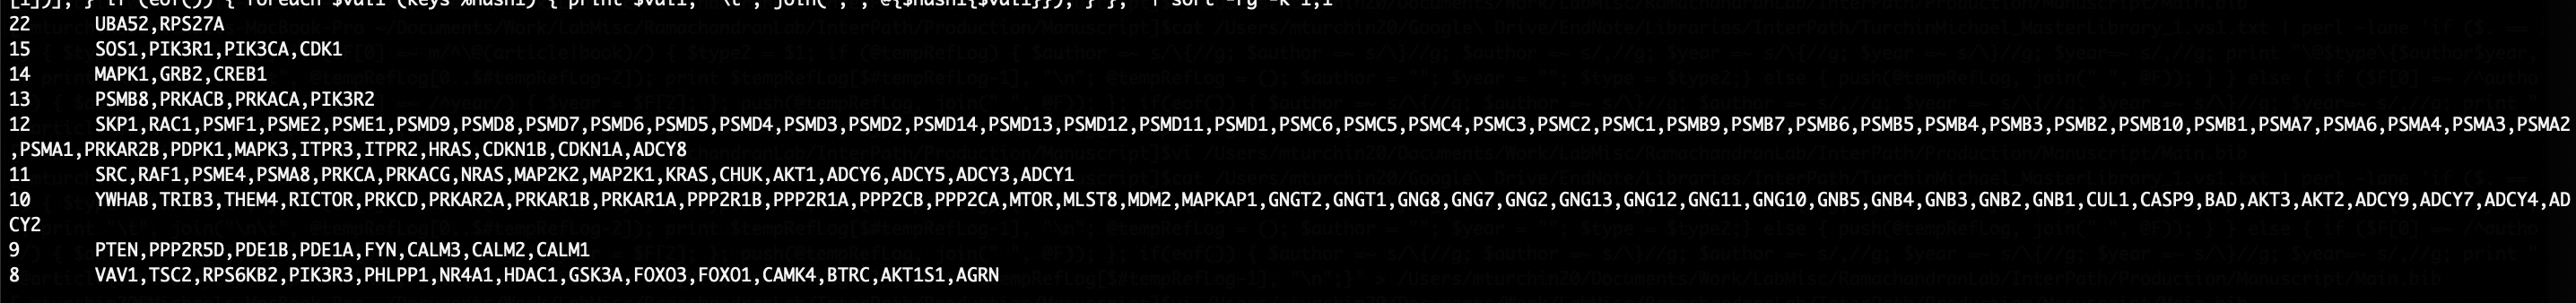
\includegraphics[scale=1]{Images/Supp/InterPath_Supp_Table_TopPathwayGeneCounts.png}
\caption[TBD]{\textbf{Table of Most Present Genes in Significant MAPIT-R Pathways} \textcolor{red}{this will be a table}}
\label{InterPath-Supp-Tables-GeneCounts}
\end{figure}
\end{landscape}
\clearpage

\begin{figure}[htbp]
\centering
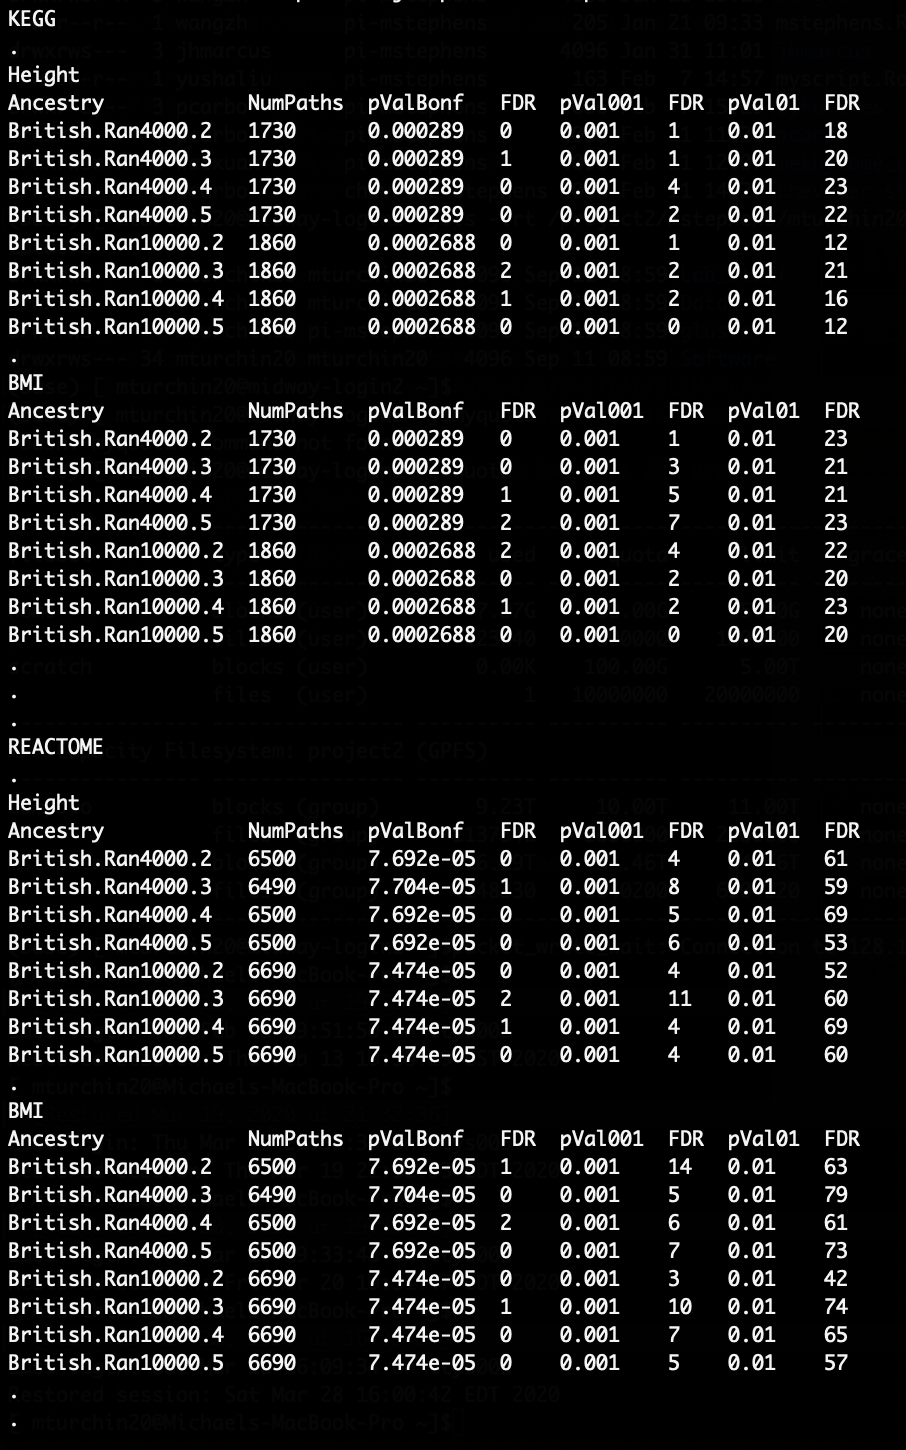
\includegraphics[scale=1.5]{Images/Supp/InterPath_Supp_Figure_FDRs_BritReps_vs1.png}
\caption[TBD]{\textbf{TBD}. }
\label{InterPath-Supp-Figure-BritReps-FDRs}
\end{figure}
\clearpage


\begingroup
\bibliographystyle{apalike}
\setstretch{1.0}
\bibliography{Main}
\endgroup


\iffalse

SCRAP

Additionally, it is unlikely that, even if such an ascertainment bias existed, it could continually be directionality consistent across pathways that span the genome. If this were an approach that aggregated single SNP tests, then directionality would not be an issue and one might become concerned about continually incorporating a persistent signal from ascertainment bias; however, because this is a joint test on multiple SNPs as once, it is far less likely that differences between genotype chip SNP distributions and non-European population SNP distributions tracts in exactly the same direction across the entire genome.

\subsubsection{Pairwise SNP Epistasis}

Our first approach to investigate SNP-level epistasis was to run the canonical pair-wise interaction model as employed by PLINK's \texttt{--epistasis} method \citep{Purcell2007} (see Online Methods and Supplementary Note for details). Here, we directly estimated the effect size of every possible SNP pairwise interaction and calculated whether it was statistically significant or not.  

Running this method on each of our four UKB population subsets, we chose to look at the 'proportion of marginally significant tests' per SNP, where marginal significance is defined as any test with a $p$-value < $1\times10^{-4}$ (Figure \ref{InterPath-Supp-Figure-PLINK}). We chose to look at proportion of tests due the varying number of SNPs across each population subset. What we find is that indeed there is variation between human ancestries in the amount of pairwise SNP epistasis across the genome. We also find that both the African and Caribbean population subsets show greater proportions of marginal interactions than the British population subset despite both non-European populations having lower sample sizes. 

\begin{figure}[t]
\centering
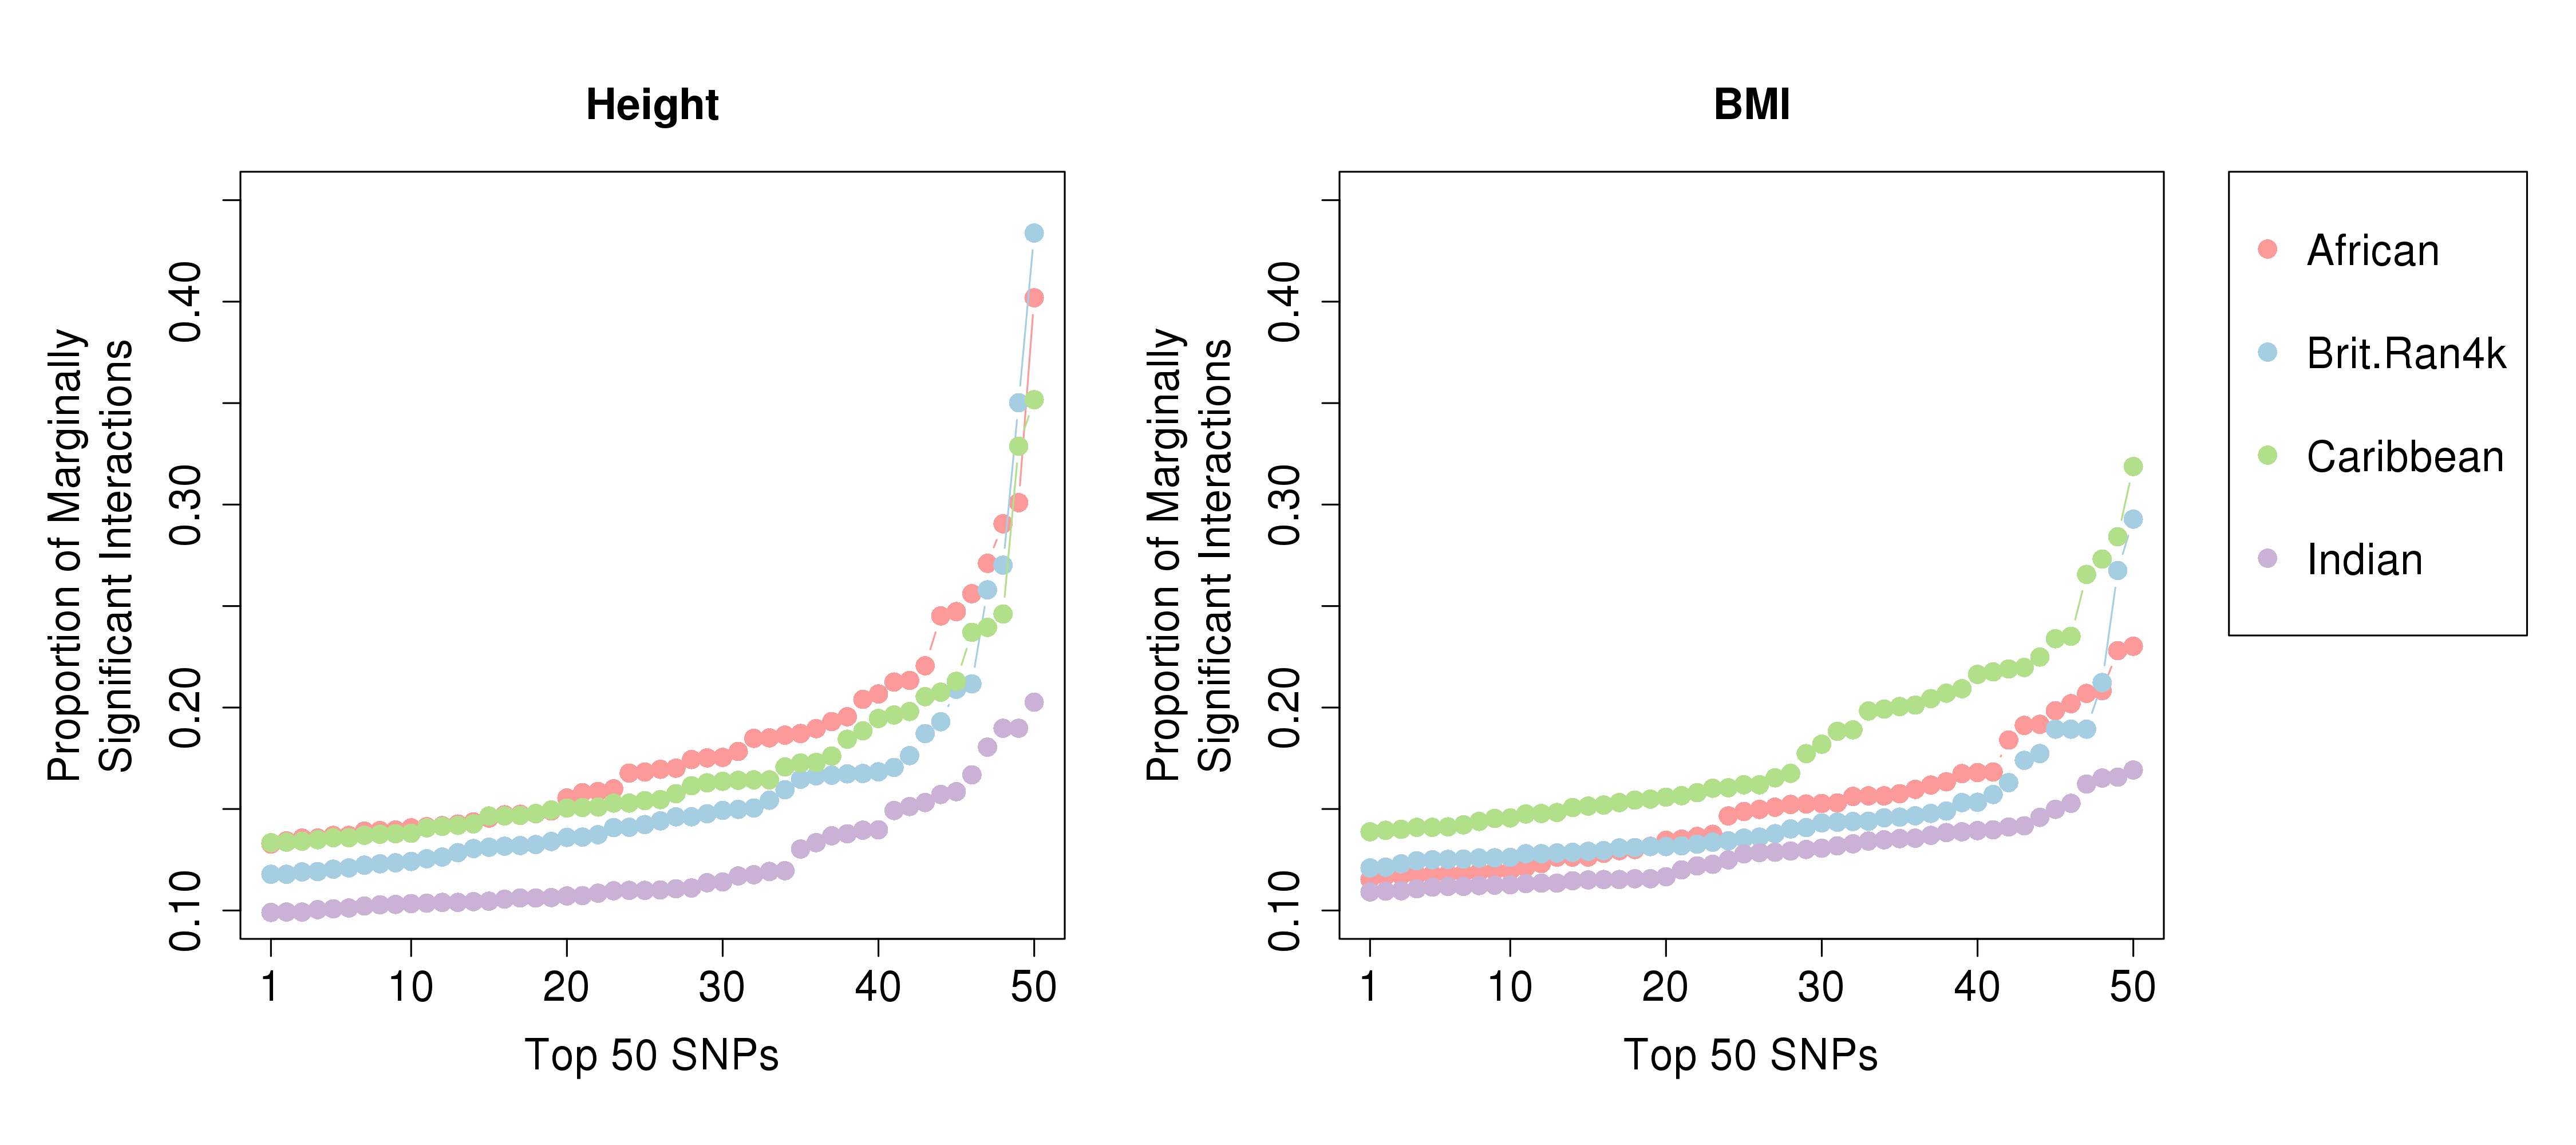
\includegraphics[scale=.35]{Images/Supp/InterPath_Supp_Figure_PLINK_vs2.png}
\caption[PLINK SNP Pairwise Epistasis]{\textbf{PLINK SNP Pairwise Epistasis.} \\ Shown are results from running PLINK's SNP-by-SNP pairwise epistasis method, \texttt{--epistasis}, on four of our initial UKB human population subsets in height and BMI. Specifically the $y$-axis shows the proportion of marginally significant interactions found per-SNP, where marginal significance is defined as the epistastic test returning a $p$-value $<$ $1\times10^{-4}$, and the $x$-axis shows the top 50 SNPs for this metric in each of the population subsets. The African subset contained 374,466 total SNPs, the British Random 4k subset contained 600,006 total SNPs, the Caribbean subset contained 410,017 total SNPs, and the Indian subset contained 505,854 total SNPs. We observe across each population different levels of marginal pairwise SNP significance as well as different patterns of significance. Additionally, both the African and Caribbean subsets contain the strongest signals.}
\label{InterPath-Supp-Figure-PLINK}
\end{figure}

\subsection{Genome Level Epistasis}\label{InterPath-Results-GenomeEpistasis}

To investigate epistasis in multiple human populations, we first extracted a variety of human ancestries from the UKB (see Online Methods). We collected a total of 8 UKB subsets with an average sample size of XXXX among the non-European populations (Supplementary Table 1), including African, Indian, Chinese, and Pakistani subsets. To maximize our sample sizes per subset, we focused on height and body mass index (BMI) as our complex traits of interest. 

The first approach we took to investigate epistasis was to look at genome-wide estimates of phenotypic PVE. Specifically, we setup a linear mixed model that incorporated both additive and epistatic interactions, and fit each of these variance components using GEMMA \citep{Zhou2012} (see Online Methods and Supplementary Note for details). Calculating these variance component PVEs for height and BMI in each of our populations, we indeed find differences across each human ancestry (Table 1).

\begin{figure}[ht]
\centering
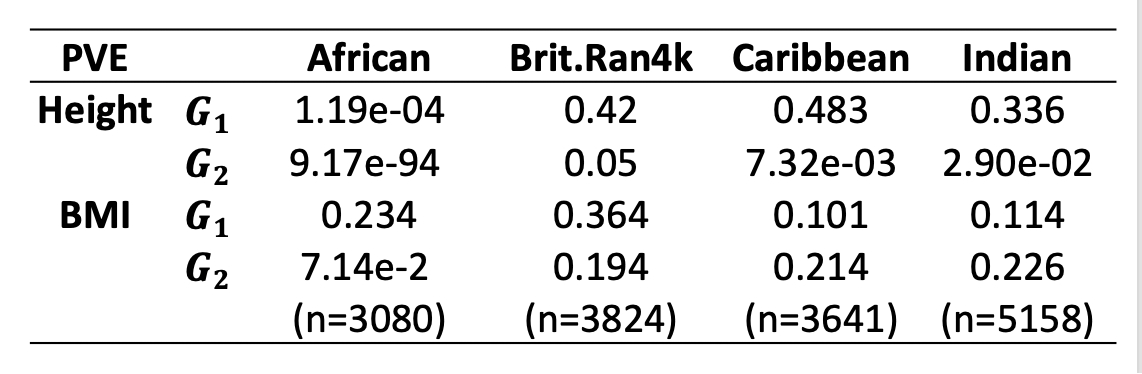
\includegraphics[scale=1]{Images/Table1_Placeholder.png}
\caption[TBD]{\textbf{TBD}. \\ this will be a table not a figure.}
\label{IntrePath-Main-Table-GEMMA}
\end{figure}

In height, we do not see anything immediately new. For the additive effects $G_1$ we mainly calculate PVEs across each population within our range of expectation (between XX and XX (citation)). Additionally, we do not currently see much evidence for second-order effects $G_2$. However, looking at BMI we see a different result. Across all populations we see non-trivial PVEs for $G_2$, ranging from XX to XX. We also see larger values in multiple non-European populations. In particular we see a particularly strong result in XXX. This might be beginning evidence that indeed, non-European populations have more potential for picking up signals of higher-order interactions in the genome.   

\fi

\end{document}
